\documentclass[12pt,UTF8]{ctexbook}
\usepackage[toc,page]{appendix}
\usepackage{array}
\usepackage{graphicx}
\usepackage{caption}
\usepackage{wrapfig}
\usepackage[table,dvipsnames]{xcolor}
\usepackage{tabularx}
\usepackage{amsmath}
\usepackage{amssymb}
\usepackage{xfrac}
\usepackage{pifont}
\usepackage{eucal}
\usepackage{titlesec}
\usepackage{amsthm}
\usepackage{tikz-cd}
\usepackage{enumitem}
\usepackage{verbatim}
\usepackage{fontspec,xunicode,xltxtra}
\usepackage{xeCJK} 
\usepackage[b]{esvect}

\definecolor{gl}{RGB}{246, 252, 240}
\definecolor{gd}{RGB}{236, 244, 230}
\definecolor{bg}{RGB}{242, 244, 228}


\setCJKmainfont[BoldFont=STZhongsong]{STSong}
\setCJKmonofont{simkai.ttf} % for \texttt
\setCJKsansfont{simfang.ttf} % for \textsf
\setlength\parskip{8pt}
\setlength{\fboxsep}{12pt}
\renewcommand\thesection{\arabic{chapter}.\arabic{section}}
\newtheorem{df}{定义}[section] 
\newtheorem{pp}{命题}[section]
\newtheorem{tm}{定理}[section]
\newtheorem{ex}{例子}[section]
\newtheorem{et}{例题}[section]
\newtheorem{sk}{思考}[section]
\newtheorem{po}{公理}
\newtheorem*{so}{解答}
\renewcommand\parallel{\mathrel{/\mskip-4mu/}}
\newcommand\dangle{%
    \mathord{\text{%
        \tikz[baseline] \draw (0.8em,0ex) -- (0.3em, 0ex) -- (.6em, 1.5ex) -- (.8em, 1.5ex) -- (.5em, 0ex) -- cycle;}}}
\newcommand\xangle{%
    \mathord{\text{%
        \tikz[baseline] \draw (0.8em,1.5ex) -- (0.3em, 0ex) -- (.64em, 0ex) -- (.8em, .36ex) -- (.42em, .36ex) -- cycle;}}}\newenvironment{proof2}{\paragraph{\textbf{证明:}}}{\hfill$\square$}
\newtheorem{xt}{习题}[section]
\newtheorem{cor}{推论}[pp]
% 列举环境的行间距
\setenumerate[1]{itemsep=0pt,partopsep=0pt,parsep=0pt,topsep=0pt}
\setitemize[1]{itemsep=0pt,partopsep=0pt,parsep=0pt,topsep=0pt}
\setdescription{itemsep=0pt,partopsep=0pt,parsep=0pt,topsep=0pt}
% 章节字体大小
\titleformat{\section}{\zihao{-2}\bfseries}{ \thesection }{16pt}{}
% 封面
\title{\zihao{0} \bfseries 第二册}
\author{\zihao{2} \texttt{大青花鱼}}
% \date{\bfseries\today}
\date{}
% 正文
\begin{document}
\maketitle
\tableofcontents
\newpage

\chapter{空间中的形状}

我们已经通过公理体系研究过平面中的简单形状,将基本的平面形和函数的图像联系起来,并且引入了向量的概念。
现在,我们进一步研究立体空间中的形状。人类生活在立体空间中,因此,研究空间中形体的性质,对我们认识世界、
改造世界有直接帮助。为了更好地理解以下的内容,我们建议你准备一把刻度尺和足够的白纸。
至于如何在纸面上画出立体形状,可以参考附录A。

\section{点、直线、平面}

和平面形一样,立体空间中的形也是从种种事物的形状总结提炼而来。平面是人类最早总结出的概念之一。
我们已经研究过平面中的形状,因此,研究立体空间时,我们把平面作为地位和点、直线相同的基本概念。

研究平面形状时,我们首先引进了公理体系。如今我们将平面公理体系扩展为立体空间的公理体系。
为此,我们要通过公设和公理定义\textbf{平面}以及它和点、直线的关系。

我们定义面为点的集合,也是线运动的结果。平面是最基本的面,一般用小写希腊字母$\alpha,\beta,\gamma$等表示。
\begin{po}{\textbf{平面公理}}\label{po:0}
    过不共线的三点,有且仅有一个平面。
\end{po}

我们也说三角形(或圆)确定一个平面。不共线的三点$A$、$B$、$C$确定的平面,可以记作平面$ABC$。

如何确定平面是“平”的呢?生活和生产中,我们一般用直线来确定一个面是不是平的。
比如,木工常常用角尺的直角边放在刨好的木板上。如果直角边总能与板面紧密贴合,就说明木板已刨平了。
水泥工用直的刮子将刚铺水泥的地面刮平。我们把人们总结出的经验作为判断平面的方法,用公理的形式确定下来。
\begin{po}{\textbf{平直公理}}\label{po:1}
    过平面上不重合两点的直线,在平面中。
\end{po}
平直公理说明,直线要么与平面没有公共点,要么只交于一点,要么全部在平面里。
直线与平面没有公共点,则称直线与平面平行,也用$\parallel$表记;直线与平面恰有一公共点,
则称直线与平面相交;直线与平面有两个或以上公共点,则称直线在平面中或平面经过直线。
用集合的语言来说,直线$l$在平面$\gamma$中,就说明$l$是$\gamma$的子集。

% 我们知道,直线把平面分为两部分,称为直线的两侧。空间中,我们把每侧称为半平面。
% 直线及其一侧的半平面构成一个展面。而每个平面又把空间分为两部分,称为平面的两方。根据实际需要,我们可以称一点在平面的上方或下方、前方或后方、左方或右方,等等。

从平面公理和平直公理,容易得到另两种定义平面的方法:
\begin{tm}\label{tm:1-0-0}
    过一条直线与该直线外一点,有且仅有一个平面。
\end{tm}
\begin{proof2}
    设直线为$l$,$P$为$l$外一点。取$l$上不同的两点,和$P$构成不共线的三点。这三点确定一个平面。
    根据平直公理,$l$在该平面中。
\end{proof2}
\begin{tm}\label{tm:1-0-1}
    过两条相交的直线,有且仅有一个平面。
\end{tm}
\begin{proof2}
    设有直线$l,m$。如果$l,m$相交,设交点为$P$,在$l,m$上各取不同于$P$的一点:$Q,R$,则$P,Q,R$不共线,
    于是确定一个平面$PQR$,根据平直公理,$l,m$都在$PQR$中。
\end{proof2}

设直线$l$与平面$\gamma$平行,没有公共点,那么它与$\gamma$中任何直线没有公共点。
比如,给定$\gamma$中一点$A$,$\gamma$中经过$A$的任何直线,都与$l$没有公共点。

平面中,两直线没有公共点,就说它们相互平行。空间中,两直线除了重合、相交和平行,还有另一种关系,
我们称之为直线\textbf{异面}。前面的例子中,根据平行公理,过$\gamma$中的点$A$,
恰有一条直线与$l$平行,其余与$l$不相交的直线,都称与$l$异面。

哪条直线与$l$平行呢?显然,在空间中,我们需要补充平行公理:
\begin{po}{\textbf{平行公理}}\label{po:2}
    过直线外一点,有且仅有一条与它平行的直线。它在直线与点确定的平面上。
\end{po}
新版的平行公理在原来的基础上,指定了平行线的位置:在直线与点确定的平面上。
换句话说,平行是一个平面内性质。两直线平行的关系必然发生在同一平面中。
也正因如此,我们把其它的无公共点的情形叫做异面。

从补充的平行公理出发,可以得到另一种定义平面的方法:
\begin{tm}\label{tm:1-0-2}
    过两条平行的直线,有且仅有一个平面。
\end{tm}
\begin{proof2}
    设直线$l \parallel m$,在$l$上找两点$P_1,P_2$,在$m$上找一点$Q$。$P_1P_2Q$确定唯一平面$\gamma$。
    在平面$\gamma$中,过$Q$作$l$的平行线。根据平行公理,这条平行线就是$m$。
    因此$l,m$共面,它们确定唯一平面$\gamma$。
\end{proof2}

再来看两个平面的关系。两个平面相交,交集是什么呢?生活中的经验告诉我们,两个平面相交,交集是直线。
比如,裁纸刀的刀面是平的,切在纸上,将纸面分成两部分,裁痕是直的。我们把这个性质用公理描述为:
\begin{po}{\textbf{交面公理}}\label{po:3}
    两个平面如果有交集,则交集至少包含两个不重合的点。
\end{po}
交面公理说明,两个平面不可能只交于一点。如果它们有两个(不重合的)公共点,那么根据平直公理,
两平面的交集包括过这两点的直线。
而如果两平面的交集中还有不属于这条直线的第三点,那么根据平面公理,这三点确定一个平面,于是两平面重合。

综上所述,从交面公理可以推出:要么两平面没有公共点,要么交集为一条直线$l$,称为两平面相交于直线$l$;
要么两平面重合。

\begin{wrapfigure}[7]{r}{0.52\textwidth} %this figure will be at the right
    \vspace{-30pt}
    \flushright
    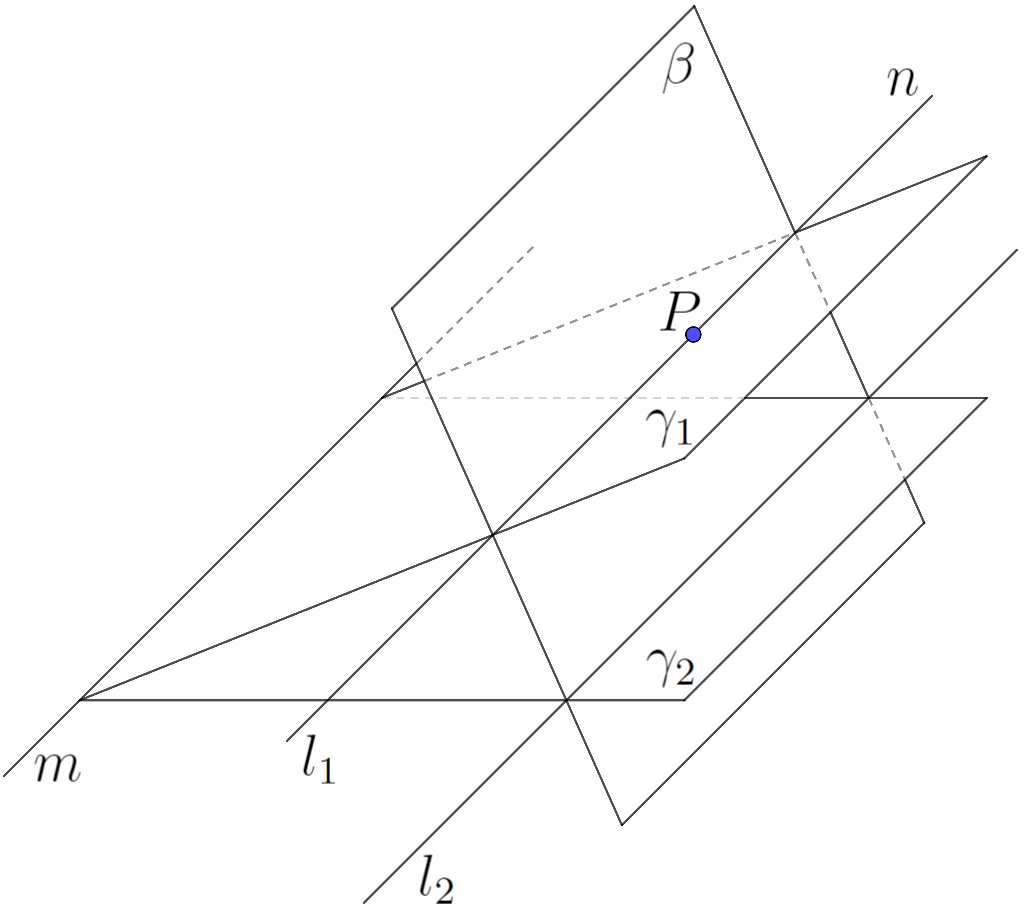
\includegraphics[width=0.5\textwidth]{三平行1.png}
\end{wrapfigure}

有了交面公理,我们可以证明空间中平行直线的递推性质。由于证明繁琐,有些地方把它当作公理引入。
\begin{tm}\label{tm:1-0-10}
    如果直线$l_1,l_2$都平行于直线$m$,那么$l_1,l_2$平行或重合。
\end{tm}
\begin{proof2}
    设$l_1,m$确定的平面为$\gamma_1$,$l_2,m$确定的平面为$\gamma_2$。分两种情况讨论:
    

    1. $\gamma_1, \gamma_2$重合。那么$l_1,l_2,m$都在此平面上。根据平面直线的结论,$l_1,l_2$平行或重合。
    
    2. $\gamma_1, \gamma_2$不重合。于是$\gamma_1\cap \gamma_2 = m$。
    取$l_1$上一点$P$,$P$与$l_2$确定平面$\beta$。$l_2\notin\gamma_1$,所以$\beta,\gamma_1$不重合。
    设$\beta\cap\gamma_1 = n$。直觉上,可以想到$n$就是$l_1$,且$n\parallel l_2$,下面来说明这两点。
    
    首先证明$n\parallel l_2$。反设$n$交$l_2$于点$Q$,则$Q\in\gamma_1\cap\gamma_2=m$,
    于是$Q\in m\cap l_2$。这与$m\parallel l_2$矛盾。因此$n\parallel l_2$。
    
    再证明$n\parallel m$。反设$n$交$m$于点$Q$,则过$Q$有$m\parallel l_2$和$n\parallel l_2$,于是$n=m$。
    但$P\in n$,因此$P\in m\cap l_1$,这与$m\parallel l_1$矛盾。因此$n\parallel m$。
    
    $n$与$l_1$都平行于$m$,且有公共点$P$,所以$n = l_1$。所以$l_1\parallel l_2$。

\end{proof2}

接下来回顾直线与平面的关系。从补充后的平行公理,可以得出直线与平面平行的判定方法:

\begin{tm}\label{tm:1-0-20}
    如果平面$\alpha$中有直线$m$平行于直线$l$,那么$l$平行于平面$\alpha$或在$\alpha$中。
\end{tm}
\begin{proof2}
    设直线$l$平行于平面$\alpha$中的某直线$m$。记$l,m$确定的平面为$\beta$。则要么$\alpha = \beta$,要么$\alpha\cap\beta = m$。如果$\alpha=\beta$,那么$l\subset\alpha$。如果$\alpha\cap\beta = m$,那么$\alpha\cap l= \beta\cap \alpha\cap l = m\cap l = \varnothing $,即$\alpha \parallel l$。
\end{proof2}
\begin{tm}\label{tm:1-0-30}
    如果直线$l$与平面$\alpha$平行,那么经过$l$的任意平面,若与$\alpha$相交,其交线也与$l$平行。
\end{tm}
\begin{proof2}
    设经过$l$的平面$\gamma$与$\alpha$交于直线$m$。一方面,$m,l$共面;另一方面$m\in\alpha$,因此$m,l$无公共点。这说明$m\parallel l$。
\end{proof2}

从这些结论可以继续推出:
\begin{tm}\label{tm:1-0-40}
    若直线$l$与平面$\alpha$平行,过$\alpha$中任一点作$l$的平行线$m$,则$m$在平面$\alpha$中。
\end{tm}
\begin{proof2}
    若直线$l$与平面$\alpha$平行,设它和$\alpha$中任一点$P$确定的平面为$\beta$,
    则$\beta$与$\alpha$相交。设交线为$m$,则$P\in m$。根据定理\ref{tm:1-0-30},$l\parallel m$。
    这就说明,过$P$而平行于$l$的直线在$\alpha$中。
\end{proof2}
\begin{tm}\label{tm:1-0-41}
    直线$l$与直线$m$平行,则过$m$的平面要么与$l$平行,要么经过$l$。
\end{tm}
\begin{proof2}
    给定过$m$的平面$\alpha$,$m\subset \alpha$与$l$平行,所以根据定理\ref{tm:1-0-20},
    $l$平行于平面$\alpha$或在$\alpha$中。
\end{proof2}

直线与平面的平行关系,也有传递性。
\begin{tm}
    若直线$l_1$与直线$l_2$平行,且与平面$\gamma$平行,则$l_2$与$\gamma$平行或在$\gamma$中。
\end{tm}
\begin{proof2}
    $l_1\parallel \gamma$。过$\gamma$中任一点作直线$n\parallel l_1$,则根据定理\ref{tm:1-0-40},
    $n$在$\gamma$中。$n\parallel l_1$,$l_1\parallel l_2$,所以根据定理\ref{tm:1-0-10},$n\parallel l_2$。
    根据定理\ref{tm:1-0-20},$l_2\parallel \gamma$或在$\gamma$中。
\end{proof2}

上面提到,两平面要么无公共点,要么相交,要么重合。我们把无公共点的平面称为\textbf{平行平面},也用$\parallel$表记。
平面中,平行公理告诉我们,过直线外一点,恰有一条直线与之平行。空间中的平面,也有类似的结论:
\begin{tm}
    过平面外一点,恰有一平面与之平行。
\end{tm}\label{tm:1-0-50}
\begin{proof2}
    设平面$\alpha$外有点$P$。在$\alpha$上选一点$A$,过$A$作两相交直线$l,m$(交点为$A$)。
    根据平行公理,过$P$恰有直线$l', m'$分别与$l,m$平行。$l',m'$相交于点$P$,确定平面$\alpha'$。
    下面证明$\alpha,\alpha'$无公共点,即$\alpha'\parallel\alpha$。

    反设$\alpha,\alpha'$有公共点。由于$P\in\alpha'$在$\alpha$外,两者不重合。
    因此根据交面公理,$\alpha \cap \alpha'$是一条直线,记为$n$。$l,m,n$共面,$l,m$相交,
    因此$l,m$中至少有一条与$n$相交。设$l$与$n$相交,交点为$Q$,则$Q\in n\subset\alpha'$。又因为$l\parallel l'$,$Q\in l$,所以$Q\notin l'$,
    因而在$\alpha'$中,过$Q$可作$l'$的平行线。但这条线在$\alpha'$中,因此不是$l$。这与平行公理矛盾。
        
    因此,$\alpha,\alpha'$无公共点,$\alpha'\parallel\alpha$。
\end{proof2}

类似的结论还有:

\begin{tm}\label{tm:1-0-60}
    过平行于平面$\alpha$的一直线$l$,恰有一平面与$\alpha$平行。
\end{tm}
\begin{proof2}
在$l$上任取一点$P$,$P\notin \alpha$,因此根据定理\ref{tm:1-0-50},
过$P$恰有一平面$\beta$与$\alpha$平行,只需证明$\beta$经过$l$。
在$\alpha$中任取一点$Q$,则根据定理\ref{tm:1-0-40},过$Q$平行于$l$的直线$m$在$\alpha$中。
$\beta$与$\alpha$平行,也就是说$\beta$与$\alpha$无公共点,
所以$\beta$与$\alpha$的子集$m$也无公共点,即$m\parallel \beta$。过$P$作$m$的平行线,
则根据定理\ref{tm:1-0-40},平行线在$\beta$中。而这条平行线就是$l$,所以$l$在$\beta$中。
这说明过$l$恰有一平面$\beta$与$\alpha$平行。
\end{proof2}

从证明中,我们还可以提炼出判定平面平行(或重合)的准则:

\begin{tm}\label{tm:1-0-70}
    给定平面$\gamma_1, \gamma_2$。设$l,m$为$\gamma_1$中的相交直线。
    若$\gamma_2$中有直线$l',m'$分别与$l,m$平行或重合,则平面$\gamma_1, \gamma_2$平行或重合。
\end{tm}
\begin{proof2}
    两平面要么相互平行,要么重合,要么相交于一直线。反设$\gamma_1, \gamma_2$相交于直线$n$。

    如果$l=l'$,那么$l\subset \gamma_1\cap\gamma_2$,于是$n=l=l'$。设$m,l$交于点$P$,$m',l'$交于点$Q$。如果$P=Q$,那么$m=m'$,于是$\gamma_1$、$\gamma_2$都是$l,m$确定的平面,$\gamma_1=\gamma_2$。如果$P\neq Q$,那么$P\notin m'$。但$P\in l=n\subset\gamma_2$,因此过$P$作$m'$的平行线,平行线应该在$\gamma_2$中,因此根据平行公理,$m$在$\gamma_2$中。这说明$\gamma_1$、$\gamma_2$都是$l,m$确定的平面,$\gamma_1=\gamma_2$。于是总有两平面重合,矛盾。

    如果$l\parallel l'$,由于$l,m,n$共面,且$l,m$相交,
    因此$l,m$中至少有一条与$n$相交。设$l$与$n$相交,交点为$Q$,则$Q\in n\subset\gamma_2$。又因为$l\parallel l'$,$Q\in l$,所以$Q\notin l'$。
    在$\gamma_2$中,过$Q$可作$l'$的平行线。但这条线在$\gamma_2$中,因此不是$l$。这与平行公理矛盾。

    因此,平面$\gamma_1, \gamma_2$平行或重合。
\end{proof2}

平行平面之间,也有类似平行直线的传递性。
\begin{tm}\label{tm:1-0-80}

如果平面$\gamma_1,\gamma_2$都平行于平面$\beta$,那么$\gamma_1,\gamma_2$平行或重合。
\end{tm}
我们先证明一个小结论:
\begin{tm}\label{tm:1-0-90}
    设平面$\gamma_1\parallel \gamma_2$。平面$\beta$与$\gamma_1,\gamma_2$相交于直线$l_1,l_2$,
    则$l_1\parallel l_2$。
\end{tm}
\begin{proof2}
    一方面,$l_1,l_2$共面。另一方面,$\gamma_1\parallel \gamma_2$说明$l_1,l_2$无公共点。
    所以$l_1\parallel l_2$。
\end{proof2}

从这个结论还可以推出:如果平面$\gamma_1\parallel \gamma_2$,那么对$\gamma_1$中任意直线,过$\gamma_2$中任一点,作它的平行线,平行线都在$\gamma_2$中。

再来证明定理\ref{tm:1-0-80}。
\begin{proof2}
    已知平面$\gamma_1,\gamma_2$都平行于平面$\beta$。在$\beta$中找一点$P$,过$P$作相交直线$l,m$。在$\gamma_1$中找一点$Q$,过$Q$分别作$l,m$的平行线$l_1,m_1$,则$l_1,m_1$都在$\gamma_1$中。它们分别是平面$\gamma_1$与$l,Q$确定的平面$\alpha_1$、平面$\gamma_1$与$m,Q$确定的平面$\alpha_2$的交线。
    设$\alpha_1,\alpha_2$分别与$\gamma_2$交于$l_2,m_2$,由于$\gamma_2\parallel \beta$,
    所以根据定理\ref{tm:1-0-30},$l_2\parallel l$,$m_2\parallel m$。因此根据定理\ref{tm:1-0-10},
    $l_2$与$l_1$平行或重合,$m_2$与$m_1$平行或重合。根据定理\ref{tm:1-0-70},$\gamma_1$、$\gamma_2$平行或重合。
\end{proof2}

最后,我们还可以得到:
\begin{tm}\label{tm:1-0-100}
    若平面$\gamma_1$与直线$l$平行,且与平面$\gamma_2$平行,则$l$与$\gamma_2$平行或在$\gamma_2$中。
\end{tm}
\begin{proof2}
    $l\parallel \gamma_1$,所以过$l$恰有一平面$\beta$与$\gamma_1$平行。如果$\beta=\gamma_2$,
    则$l\subset\gamma_2$。如果$\beta\parallel\gamma_2$,那么$l\parallel \gamma_2$。
    如果$\beta$与$\gamma_2$相交于直线$m$,那么由于$m,l$共面且无公共点,$m\parallel l$。
    于是,根据定理\ref{tm:1-0-20},$l\parallel \gamma_2$或在$\gamma_2$中。
\end{proof2}

总结:

我们初步建立了关于空间形状的公理体系,引入了空间中平面的概念,并界定了点、直线和平面的关系:
\begin{enumerate}
    \item 直线和平面都是点的集合。
    \item 直线可能与平面平行、相交,或在平面中。
    \item 直线可能与直线异面、平行、相交、重合。
    \item 平面可能与平面平行、相交、重合。
    \item 直线与直线相交于一点,直线与平面相交于一点,平面与平面相交于一直线。
\end{enumerate}


\begin{sk}
    \mbox{} \\
    \indent 1. 定理\ref{tm:1-0-100} 的证明中,我们讨论了$\beta$与$\gamma_2$相交于直线$m$的情形。实际上$\beta$是否会与$\gamma_2$相交?如何看待这个论证?
\end{sk}

\begin{xt}
    \mbox{} \\
    \indent 1. 证明:如果直线$l$与直线$m$平行,那么过$l$的平面与过$m$的平面要么平行,要么重合,
    要么交于$l,m$之一,要么交于与$l,m$都平行的直线$n$。 
\end{xt}


\section{空间向量}

上一节中,我们使用公理体系讨论空间中的形状。可以看到,使用公理体系讨论虽然严谨,但过于抽象,步骤繁琐。
仅处理点线面的平行关系,就需要大量的篇幅。为此,我们尝试用向量的概念来讨论空间中的形状。

平面中,我们用向量表示点,以及原点到此点的平移。现在我们把向量的概念扩展到空间中。
我们把空间看作集合,记为$\mathbb{V}$,其中的元素称为向量或点。向量满足如下规则:

\begin{enumerate}
    \item 加法结合律:$\forall \,\, \mathbf{a}, \mathbf{b}, \mathbf{c} \in \mathbb{V}$,$\mathbf{a}+ (\mathbf{b} + \mathbf{c}) = (\mathbf{a} + \mathbf{b}) + \mathbf{c}$。
    \item 加法交换律:$\forall \,\, \mathbf{a}, \mathbf{b} \in \mathbb{V}$,$\mathbf{a} + \mathbf{b} = \mathbf{b} + \mathbf{a}$。
    \item 存在零向量:$\forall \,\, \mathbf{a} \in \mathbb{V}$,$\mathbf{a} + \mathbf{0} = \mathbf{a}$。
    \item 放缩和四则运算相容:$\forall \,\, \mathbf{a} \in \mathbb{V}$,$1\cdot \mathbf{a} = \mathbf{a}$。$\forall s, t \in \mathbb{R}$,$(s + t)\cdot\mathbf{a} = (s\cdot\mathbf{a}) + (t\cdot\mathbf{a})$,$(s \cdot t)\cdot \mathbf{a} = s \cdot (t\cdot \mathbf{a})$。
    \item 放缩和平移相容:$\forall \,\, \mathbf{a}, \mathbf{b} \in \mathbb{V}$,$\forall \,\, t \in \mathbb{R}$,$t\cdot(\mathbf{a} + \mathbf{b}) = t\cdot\mathbf{a} + t\cdot\mathbf{b}$。
\end{enumerate}

这个定义与平面向量相同。在此基础上,我们用同样的方式定义直线、线段和射线。
\begin{df}
    过原点的直线是非零向量放缩得到的集合。不过原点的直线是过原点的直线按一点平移得到的集合。
\end{df}
给定非零向量$A = \mathbf{a}$,$ \{t\mathbf{a} \, | \, t\in\mathbb{R}\}$是一条过原点$O$和$A$的直线$OA$,
称为$A$\textbf{引出}的直线,记为$\mathbb{R}\mathbf{a}$。$\mathbf{a}$称为直线的\textbf{方向向量}。
给定向量$B = \mathbf{b}$,$ \{t\mathbf{a}+\mathbf{b} \, | \, t\in\mathbb{R}\}$是一条方向为$\mathbf{a}$且经过$B$的直线,
记为$\mathbb{R}\mathbf{a}+\mathbf{b}$,其中$\mathbb{R}\mathbf{a}$称为它的\textbf{线性部分};
而$ \{t\mathbf{a}+(1 - t)\mathbf{b} \, | \, t\in\mathbb{R}\}$就是直线$AB$。

给定非零向量$\mathbf{a}$,如果向量$\mathbf{b}$可以通过$\mathbf{a}$放缩得到,
或者说$\mathbf{b}\in \mathbb{R}\mathbf{a}$,就称两者\textbf{共线}。

类比可以定义线段和射线:给定非零向量$A = \mathbf{a}$和向量$B =\mathbf{b}$,
$ \{(1 - t)\mathbf{a}+t\mathbf{b} \, | \, t\in [0, 1]\}$是线段$AB$,
$ \{(1 - t)\mathbf{a}+t\mathbf{b} \, | \, t \geqslant 0 \}$是射线$AB$。

\begin{figure}[h] 
    % \vspace{-4pt}
    \centering
    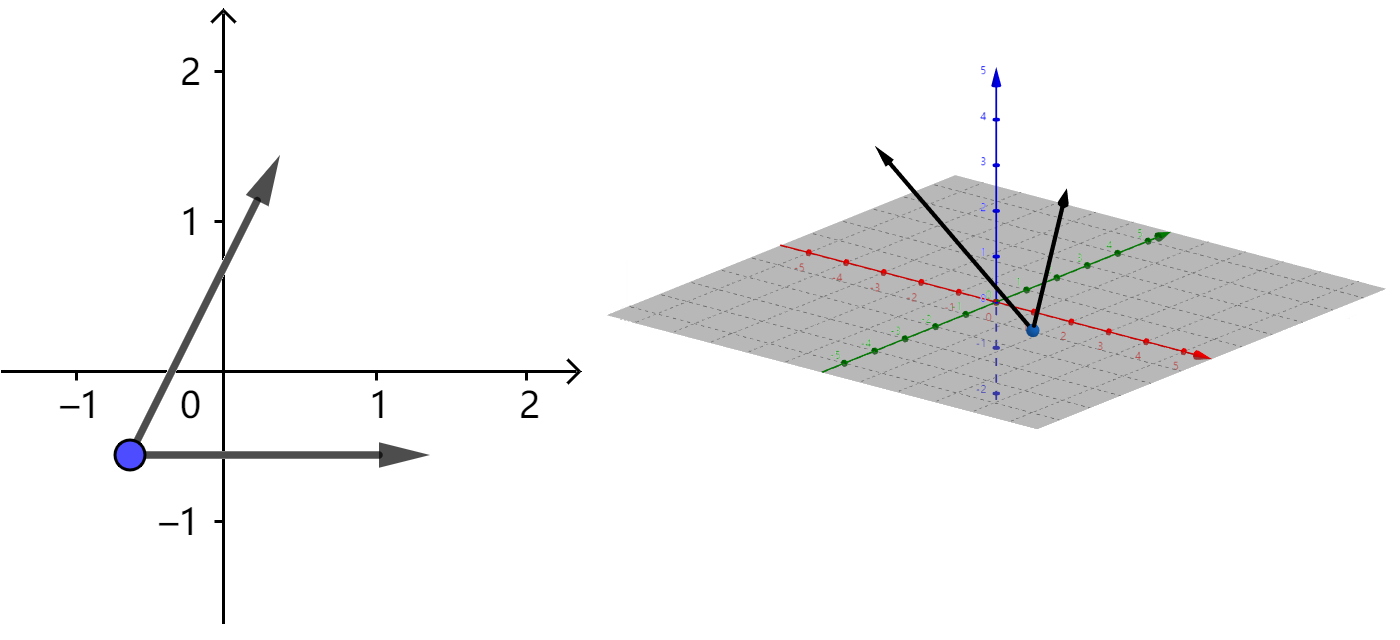
\includegraphics[width=0.8\textwidth]{平面和空间向量1.png}
    \caption*{\texttt{平面和立体空间中的向量}}
\end{figure}

空间向量与平面向量的唯一不同的地方在于,空间向量遵循的不再是平面的根本性质,
而是空间的根本性质。为了描述空间的根本性质,我们首先引进线性相关的概念:
\begin{df}
    给定$n$个向量$\mathbf{a}_1, \mathbf{a}_2, \cdots , \mathbf{a}_n$,
    对实数$t_1, t_2, \cdots , t_n$来说,
    $t_1\mathbf{a}_1 + t_2\mathbf{a}_2 + \cdots + t_1\mathbf{a}_n$称为这$n$个向量的\textbf{线性组合}。
    如果存在一组不全为零的实数$t_1, t_2, \cdots , t_n$,
    使得线性组合$t_1\mathbf{a}_1 + t_2\mathbf{a}_2 + \cdots + t_1\mathbf{a}_n$是零向量,
    就说这$n$个向量\textbf{线性相关}。如果不存在这样一组实数,就说这$n$个向量\textbf{线性无关}。
\end{df}

举例来说,单个非零向量总是线性无关的,因为非零实数乘以非零向量总得到非零向量。
又如:如果有不全为零的实数$t_1,t_2$使得平面向量$A, B$的线性组合:$t_1A + t_2B$等于零向量,就说$A, B$线性相关。

具体来说,平面直角坐标系中,令$\mathbf{e}_1=(1,0)$,$\mathbf{e}_2=(0,1)$。
如果$A = 2\mathbf{e}_1 - \mathbf{e}_2$,$B = -6\mathbf{e}_1 + 3 \mathbf{e}_2$,那么
$$3A + B = \mathbf{0}.$$
也就是说,选取$t_1 = 3$,$t_2 = 1$,就使得线性组合:$t_1A + t_2B$等于零向量。因此,以上两个向量$A, B$线性相关。

设$A = 2\mathbf{e}_1 - \mathbf{e}_2$,$B = \mathbf{e}_1 + 3 \mathbf{e}_2$,那么对任何$t_1,t_2$,线性组合$t_1A + t_2B$可以写为:
\begin{align}
t_1A + t_2B &= t_1 \left( 2\mathbf{e}_1 - \mathbf{e}_2 \right) + t_2 \left( \mathbf{e}_1 + 3 \mathbf{e}_2 \right) \notag \\
&= (2t_1 + t_2) \mathbf{e}_1 + (-t_1 + 3t_2)\mathbf{e}_2.\notag
\end{align}
要使得$t_1A + t_2B$为零向量$(0,0)$,就要求它的横坐标和纵坐标同时为零。也就是说,$t_1,t_2$应该是二元一次方程组
$$
\left\{
\begin{array}{cl}
  2t_1 + t_2 &= 0 \\
  -t_1 +3t_2 &= 0 \\
\end{array}
\right.
$$
的解。解这个二元一次方程组,得到$t_1=t_2=0$。也就是说,不存在不全为零的实数$t_1, t_2$,
使得线性组合$t_1A + t_2B$为零向量。我们说$A, B$线性无关。

以上的例子也给出了判断一组向量是否线性相关的方法。
我们将“线性组合$t_1\mathbf{a}_1 + t_2\mathbf{a}_2 + \cdots + t_1\mathbf{a}_n$是零向量”
的条件转化为关于$t_1, t_2, \cdots , t_n$的多元一次方程组。如果方程组的解集中有不全为零的解,
这组向量就线性相关。如果方程组没有不全为零的解,就说这组向量线性无关。

直观来看,两个平面向量线性相关和共线是一回事。$A, B$线性相关,
就是说有有不全为零的实数$t_1,t_2$使得$t_1A + t_2B$等于零向量。
不妨设$t_1$不为零,那么$A = -\frac{t_2}{t_1}B$,因此$A\in\mathbb{R}B$,即$A, B$共线。
反之亦然。平面的根本性质告诉我们,存在两个不共线的向量,也就是说,
不多于两个平面向量,可以线性无关。

如果向量多于两个,平面的根本性质告诉我们,只要其中两个向量$A, B$不共线,
其余的向量都可以都可以表示成$sA + tB$的形式。
因此,设有平面向量$\mathbf{a}_1, \mathbf{a}_2, \cdots , \mathbf{a}_n$。
如果$\mathbf{a}_1, \mathbf{a}_2$共线,那么它们线性相关,存在$t_1\mathbf{a}_1 + t_2\mathbf{a}_2 = \mathbf{0}$。于是
$$t_1\mathbf{a}_1 + t_2\mathbf{a}_2 + \sum_{i>2}0\cdot\mathbf{a}_i = \mathbf{0}.$$
如果$\mathbf{a}_1, \mathbf{a}_2$不共线,那么根据平面的根本性质,$\mathbf{a}_3$可以写成:
$$ \mathbf{a}_3 = s\mathbf{a}_1 + t\mathbf{a}_2.$$
于是
$$s\mathbf{a}_1 + t\mathbf{a}_2 - 1\cdot\mathbf{a}_3 + \sum_{i>3}0\cdot\mathbf{a}_i = \mathbf{0}.$$
也就是说,多于两个平面向量总线性相关。

这个结论反映了平面向量的本质:可以选出两个向量,所有向量都可以从它们开始,通过平移、放缩得到。
这两个向量叫作平面的基底。而空间中的点显然不一定在同一个平面里。我们把平面的根本性质替换为\textbf{空间的根本性质}:

\begin{enumerate}
    \item 给定一个非零向量,总能找到另一个向量,使得两者线性无关。
    \item 给定两个线性无关的向量,总能找到另一个向量,使得三者线性无关。
    \item 从线性无关的向量$A, B, C$出发,经过放缩、平移,可以得到空间中任何向量。具体来说,
    任何向量都可以表示成$sA + tB + uC$的形式,集合$\{sA + tB + uC \, | \, s, t, u \in\mathbb{R}\}$就是整个空间。
    这样的$A, B, C$称为空间的一组\textbf{基}或\textbf{基底}。
\end{enumerate}

对比平面和空间的根本性质,可以发现,主要的变化是“$2$变成$3$”。平面中保证存在两个线性无关的向量,
空间中保证存在三个线性无关的向量。按照类似的推理,我们可以得到结论:不多于三个空间向量,
可以线性无关;多于三个空间向量,总是线性相关。我们把这个数字称为\textbf{维数}。平面的维数是$2$,立体空间的维数是$3$。

与平面向量一样,给定基底后,任一空间向量$\mathbf{a}$可以唯一地写成基向量的线性组合:
$$ \mathbf{a} = a_x\mathbf{e}_x + a_y\mathbf{e}_y + a_z\mathbf{e}_z.$$
其中$a_x, a_y, a_z$是实数。$(a_x, a_y, a_z)$称为$\mathbf{a}$的\textbf{坐标},
$a_x, a_y, a_z$称为它的\textbf{坐标分量}。

于是我们可以定义立体空间中的平面:
\begin{df}
    过原点的平面是两个线性无关的向量通过平移、放缩得到的集合。不过原点的平面是过原点的平面按一点平移得到的集合。
\end{df}

\begin{figure}[h] 
    % \vspace{-4pt}
    \centering
    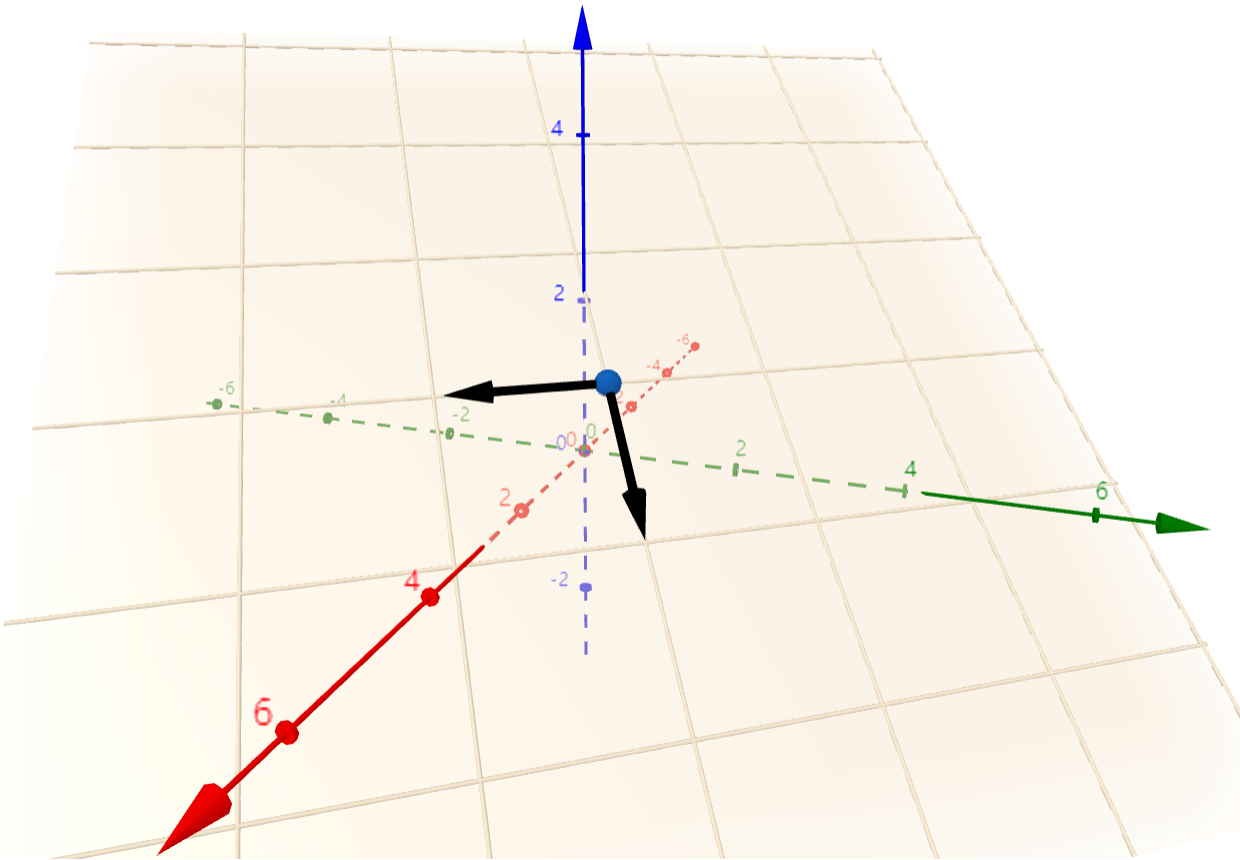
\includegraphics[width=0.5\textwidth]{空间基底1.png}
    \caption*{\texttt{从向量到平面}}
\end{figure}

给定线性无关的向量$A = \mathbf{a}, B = \mathbf{b}$,$ \{s\mathbf{a} + t\mathbf{b} \, | \, s, t\in\mathbb{R}\}$是一个过原点$O$和$A, B$的平面$OAB$,
也称为向量$\mathbf{a},\mathbf{b}$\textbf{生成}的平面,简记为$\mathbb{R}\mathbf{a}+\mathbb{R}\mathbf{b}$。
$\mathbf{a},\mathbf{b}$也称为$\mathbb{R}\mathbf{a}+\mathbb{R}\mathbf{b}$的\textbf{生成向量}。
给定向量$C = \mathbf{c}$,$ \{s\mathbf{a}+t\mathbf{b}+\mathbf{c}\, | \, s,t\in\mathbb{R}\}$是一个过$C$的平面,
也记为$\mathbb{R}\mathbf{a}+\mathbb{R}\mathbf{b}+\mathbf{c}$。$\mathbb{R}\mathbf{a}+\mathbb{R}\mathbf{b}$称为它的\textbf{线性部分}。
而$ \{s\mathbf{a}+t\mathbf{b}+(1 - s - t)\mathbf{c} \, | \, t\in\mathbb{R}\}$就是过$A,B,C$的平面$ABC$。

来看几个具体的例子。选定空间的一组基底$\mathbf{e}_x,\mathbf{e}_y,\mathbf{e}_z$,
我们可以构建坐标系$Oxyz$,其中$x$轴、$y$轴、$z$轴分别是基向量引出的直线$\mathbb{R}\mathbf{e}_x$、
$\mathbb{R}\mathbf{e}_y$、$\mathbb{R}\mathbf{e}_z$。空间中任一点$A$的坐标是$(a_x,a_y,a_z)$。
$x$轴、$y$轴构成平面:
$$ Oxy : \{s\mathbf{e}_x+t\mathbf{e}_y\,|\,s,t\in\mathbb{R}\} = \mathbb{R}\mathbf{e}_x + \mathbb{R}\mathbf{e}_y. $$
$x$轴、$z$轴构成平面:
$$ Oxz : \{s\mathbf{e}_x+t\mathbf{e}_z\,|\,s,t\in\mathbb{R}\} = \mathbb{R}\mathbf{e}_x + \mathbb{R}\mathbf{e}_z. $$
$y$轴、$z$轴构成平面:
$$ Oyz : \{s\mathbf{e}_y+t\mathbf{e}_z\,|\,s,t\in\mathbb{R}\} = \mathbb{R}\mathbf{e}_y + \mathbb{R}\mathbf{e}_z. $$
给定点$A(3,0,0)$、$B(0,2,0)$、$C(0,0,1)$,则经过它们的平面为:
$$ \{sA+tB+(1 - s - t)C \, | \, t\in\mathbb{R}\} = \{(3s,\,2t,\,1-s-t) \, | \, t\in\mathbb{R}\}. $$

可以验证,这样定义的点、直线、平面符合上一节中的各个公理(见附录B)。

\begin{sk}
    \mbox{}  \\
    \indent 1. 张三这样总结空间向量的特性:一个向量平移缩放得到一条直线;两个向量平移缩放可以得到一个平面;
    三个向量平移缩放可以得到整个空间。怎么看待这个说法?\\
    \indent 2. 是否有维数大于$3$的空间?如何在这样的空间中定义向量?这样定义的向量和空间和$2$维、$3$维的向量有什么相同和不同之处?
\end{sk}

\begin{xt}
    \mbox{}  \\
    \indent 1. 证明:如果一组线性无关的向量的线性组合等于零向量,那么线性组合中每个向量的系数都是$0$。\\
    \indent 2. 证明:给定空间一组基底,空间中每个向量都可以唯一写成基向量的线性组合。\\
    \indent 3. 判断以下向量是否线性相关:\\
    $$
    \begin{array}{ll}
        \mbox{\ding{172}}.\,\,\, (1,2,3),\,\,\,(4,5,6), \,\,\,(7,8,9) \quad & \mbox{\ding{173}}.\,\,\, (1,0,-1),\,\,\, (1,2,0) \,\,\,(-2,2,3)  \\
        \mbox{\ding{174}}.\,\,\, (2,1,-1), \,\,\, (2,-5,-7), \,\,\,(1,-1,-2) \quad & \mbox{\ding{175}}.\,\,\, (a,0,b),\,\,\, (b,-a,0) \,\,\,(a,b,0) 
    \end{array}
    $$
    \indent 4. 已知直线$\mathbb{R}\mathbf{a}+\mathbf{b}$和直线外一点$P$,如何表示它们确定的平面?\\
    \indent 5. 一直两条直线相交于点$P$,方向向量分别是$\mathbf{a},\mathbf{b}$,如何表示这两条直线,以及它们确定的平面?\\
    \indent 6. 设有向量$\mathbf{a}=(0,1,1)$、$\mathbf{b}=(2,-1,0)$、$\mathbf{c}=(1,1,-1)$。
    平面$\gamma = \{s\mathbf{a} + t\mathbf{b} + \mathbf{c} \, | \, s,t,\in\mathbb{R}\}$。\\
    \indent 6.1. 判断点$(5,1,-2)$、$(3,2,1)$、$(0,5,0)$是否在平面上。\\
    \indent 6.2. 点$(1,0,0)+u(0,-1,3)$在平面$\gamma$中,求它的坐标。\\
    \indent 6.3. 直线$l$在平面$\gamma$中,证明:它的方向向量是$\mathbf{a},\mathbf{b}$的线性组合。
\end{xt}

\section{角度和长度}
我们可以通过向量引进空间中角度、长度和距离的概念。和平面中一样,
我们选定空间的一组基底$\mathbf{e}_x,\mathbf{e}_y,\mathbf{e}_z$,然后定义內积:
$$
\begin{array}{c}
    \forall  A = a_x\mathbf{e}_x+a_y\mathbf{e}_y+a_z\mathbf{e}_z,\,\,B = b_x\mathbf{e}_x+b_y\mathbf{e}_y+b_z\mathbf{e}_z, \notag \\
     A\cdot B = a_xb_x + a_yb_y + a_zb_z. \notag
\end{array}
$$ 
如果向量$A,B$的內积等于$0$,就说它们垂直。我们定义向量$A$的长度为
$$\|A\| = \sqrt{A\cdot A} = \sqrt{a_x^2 + a_y^2 + a_z^2},$$
长度为$1$的向量称为\textbf{单位向量}。任何非零向量除以自己的长度,都得到一个与自己共线的单位向量。
我们把这个操作称为\textbf{向量的归一}。

两点$A,B$之间的距离是:
$$\|A-B\| = \sqrt{(A - B)\cdot(A-B)} = \sqrt{(a_x - b_x)^2 + (a_y-b_y)^2 + (a_z-b_z)^2}. $$

平面向量的内积,小于等于长度之积。空间向量也有类似的性质:
\begin{align}
    &(a_x^2 + a_y^2 + a_z^2)(b_x^2 + b_y^2 + b_z^2) \notag \\
    =\,\,& (a_xb_x + a_yb_y + a_zb_z)^2 + (a_xb_y - a_yb_x)^2 + (a_xb_z - a_zb_x)^2 + (a_yb_z - a_zb_y)^2 \notag \\
    \geqslant\,\,& (a_xb_x + a_yb_y + a_zb_z)^2 \notag 
\end{align}
这个不等式也称为\textbf{内积不等式}。由此,类比平面向量,我们可以定义\textbf{空间向量的夹角}:
$$ \cos \angle AOB = \frac{a_xb_x + a_yb_y + a_zb_z}{\sqrt{(a_x^2 + a_y^2 + a_z^2)(b_x^2 + b_y^2 + b_z^2)}}$$
直线是非零向量放缩的结果,所以,可以定义空间中两条直线的夹角为它们的方向向量的夹角。

向量$A,B$垂直时,$\cos \angle AOB = 0$,即夹角为$90^\circ$。
向量夹角为$0^\circ$、$180^\circ$时,两向量共线,两直线同向或反向。
要注意的是,空间中,我们无法定义两向量夹角的方向。

\begin{sk}
    \mbox{} \\
    \indent 1. 内积不等式取等号的条件是什么?如何从直观上理解?\\
    \indent 2. 平面中,向量夹角的正弦与向量长度的乘积对应着向量的面积。
    立体空间中,是否可以作类似的定义?如何从直观上理解?
\end{sk}

\begin{xt}
    \mbox{} \\
    \indent 1. 已知向量$A(-1, 3, 1)$、$B(1, 2, 0)$,求它们的长度、内积和夹角。它们是否垂直?\\
    \indent 2. 已知向量$A(-2.4, 0, 1)$、$B(0.5, 1, 1.2)$,求它们的长度、内积和夹角。它们是否垂直?\\
    \indent 3. 已知直线$l_1: \mathbb{R}(1,2,-2.5) + (0,-1,-1)$、$l_2: \mathbb{R}(2,0,0.8) + (-2.5,1.1,1.7)$,
    求两直线的夹角。它们是否垂直?是否有公共点?\\
    \indent 4. 已知向量$A(2, 0, 1)$,求与$A$夹角为$60^\circ$的单位向量。
\end{xt}

\section{垂直和投影}

通过内积,我们已经定义了空间向量以及直线间的垂直关系。
下面来看直线与平面的垂直关系。直线与平面垂直,是直线与平面相交的特殊情形。
\begin{df}\label{df:1-3-10}
    给定直线$l$和平面$\gamma$,如果$\gamma$中任意直线都与$l$垂直,就说平面$\gamma$与$l$垂直。
\end{df}
用向量的语言来说,直线垂直于平面,即垂直于它的线性部分中的所有向量。

给定了直线和平面,如何判定它们垂直呢?我们从以下基本性质出发:
\begin{tm}\label{tm:1-3-10}
    如果向量$\mathbf{a}$垂直于另两个向量$\mathbf{u},\mathbf{v}$,
    那么$\mathbf{a}$也与$\mathbf{u},\mathbf{v}$的任何线性组合垂直。
\end{tm}
\begin{proof2}
    如果$\mathbf{a}\perp \mathbf{u}$、$\mathbf{a}\perp \mathbf{v}$,按照定义,
    $$ \mathbf{a}\cdot \mathbf{u} = 0, \quad \mathbf{a}\cdot \mathbf{v} = 0. $$
    于是,$\forall s, t\in\mathbb{R}$,
    \begin{align}
        \mathbf{a}\cdot (s\mathbf{u} + t\mathbf{v}) = s\mathbf{a}\cdot \mathbf{u} + t\mathbf{a}\cdot \mathbf{v} = 0. \notag
    \end{align}
\end{proof2}

给定直线$l$和平面$\gamma$中两条相交直线。设$l$的方向向量为$\mathbf{a}$,
两条相交直线相交于点$P$,方向向量为线性无关的向量:$\mathbf{u},\mathbf{v}$,那么$\gamma$可以表示成
$$ \gamma = \{s\mathbf{u} + t\mathbf{v} + P \, | \, s,t\in\mathbb{R}\} = \mathbb{R}\mathbf{u} + \mathbb{R}\mathbf{v} + P. $$
因此,$\gamma$中任一直线的方向向量总是$\mathbf{u},\mathbf{v}$的线性组合。
如果$\mathbf{a}$垂直于$\mathbf{u},\mathbf{v}$,那么根据定理\ref{tm:1-3-10},
$l$垂直于$\gamma$中任一直线,因而垂直于平面$\gamma$。我们可以把这个结论总结为:
\begin{tm}\label{tm:1-3-20}
    直线与平面垂直,当且仅当它垂直于平面中两条相交直线。
\end{tm}
接下来我们自然要问:给定了平面,是否有与它垂直的直线呢?

从以上的讨论来看,关键是找到与平面中两个线性无关的向量都垂直的向量。

首先来看平面中的情况。给定非零平面向量$A$,是否有(非零)向量与它垂直?
根据平面的根本性质,总存在与$A$不共线的向量$B$。但$B$不一定与$A$垂直。
下面我们从$B$出发,找一个与$A$垂直的非零向量。

直观上,向量$A,B$确定一个平行四边形,我们将它沿着$A$的方向“平推”,可以把它“扶正”,变成一个矩形。
矩形的另一边就和$A$垂直了。把这个想法用向量表示,我们考虑向量$B' = B + uA$,其中$u\in\mathbb{R}$是系数。
$B'$是$B$沿$A$方向移动得到的。我们希望$B'\perp A$,即内积为$0$:
$$ A\cdot B = A\cdot (B + uA) = 0$$
解得$u = -\frac{A\cdot B}{A\cdot A}$。
这样我们就找到了垂直于$A$的非零向量$B' = B -\frac{A\cdot B}{A\cdot A}A$。

直观来看,过$B$作直线$OA$的垂线,设垂足为$P$,则$\frac{A\cdot B}{A\cdot A}A$就是向量$OP$。
如果想象$OA$为水平线,线段$OB$是一根杆子,那么线段$OP$可以看成$OB$在竖直照射的阳光下的影子。
我们把向量$\vv{OP}$称为向量$\vv{OB}$在直线$OA$上的投影。严格的定义如下:
\begin{df}\label{df:1-3-20}
    给定向量$\mathbf{a}$和向量集合$S$。如果向量$\mathbf{y}\in S$使得$\mathbf{a} - \mathbf{y}$垂直于
    $S$中所有向量,就说$\mathbf{y}$是$\mathbf{a}$在$S$中的\textbf{投影},
    $\mathbf{a} - \mathbf{y}$是$\mathbf{a}$关于$S$的\textbf{修正}。
\end{df}
按照严格的定义,向量$\vv{OP}$就是向量$\vv{OB}$在直线$OA$中的投影。
从$\vv{OB}$中减去它在直线$OA$上的投影,得到垂直于$\vv{OA}$的向量(或者说关于直线$OA$的修正),
这种方法叫做\textbf{消影法}。

我们可以进一步将$A$和$B'$分别归一,就得到两个相互垂直的单位向量。
我们把这样两个向量称为平面的\textbf{正交归一基}。注意到$A,B$是平面的一组基底。
从$A,B$出发得到正交归一基,这个过程称为\textbf{基底的正交归一}。

空间的根本性质告诉我们,给定两个线性无关的向量$A,B$,总有向量$C$使得$A,B,C$为空间的基底。
我们尝试用消影法将它正交归一,得到空间的正交归一基$A_1,B_1,\mathbf{n}$,然后证明$\mathbf{n}$与$A,B$垂直。

\begin{figure}[h] 
    % \vspace{-4pt}
    \centering
    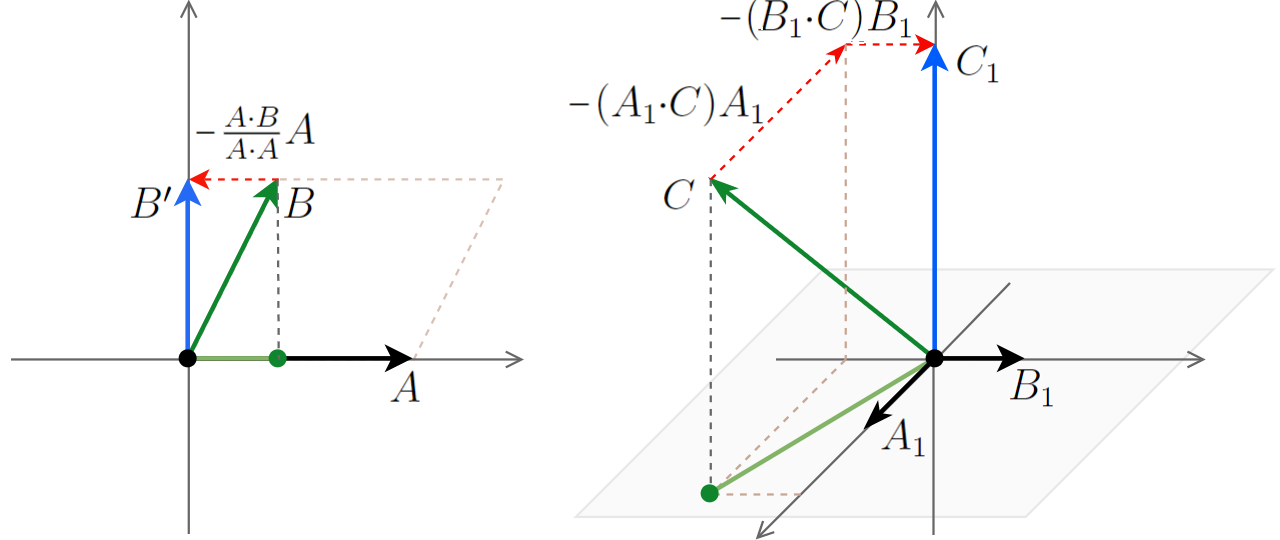
\includegraphics[width=0.8\textwidth]{消影法1.png}
    \caption*{\texttt{平面和立体空间中的消影法}}
\end{figure}

根据已知条件,$A,B$确定一个平面$\gamma$,而且是平面$\gamma$的基底。用消影法将$A,B$正交归一,
得到平面$\gamma$的正交归一基$A_1,B_1$。然后再次使用消影法。这次我们要消去$C$在平面$\gamma$中的投影。
考虑向量$C_1=C+uA_1+vB_1$,其中$u,v$是未知系数。
我们希望$C_1$与$A_1,B_1$垂直。分别计算内积$A_1\cdot C_1$、$B_1\cdot C_1$,两者都应当等于$0$。
于是得到关于$u,v$的方程组:
$$
    \left\{
    \begin{array}{cl}
    A_1\cdot C + u\|A_1\|^2 + vA_1\cdot B_1 &= 0 \\
    B_1\cdot C + uA_1\cdot B_1 + v\|B_1\|^2 &= 0 \\
    \end{array}
    \right.
$$
$A_1,B_1$为正交归一基,所以$A_1\cdot B_1 = 0$,$\|A_1\|^2 = \|B_1\|^2 = 1$。因而解得:
$$
    \left\{
    \begin{array}{cl}
    u &= -A_1\cdot C \\
    v &= -B_1\cdot C \\
    \end{array}
    \right.
$$
这样我们就得到了与$A_1,B_1$都垂直的向量
$$ C_1 = C - (A_1\cdot C)A_1 - (B_1\cdot C)B_1. $$
它是从$C$中去掉它在平面$\gamma$中的投影$(A_1\cdot C)A_1 + (B_1\cdot C)B_1$得到的。
将它归一,就得到垂直于$A_1,B_1$的单位向量:$\mathbf{n} = \frac{C_1}{\|C_1\|}$ 。
于是我们得到了空间的正交归一基:$A_1,B_1,\mathbf{n}$。

$A_1,B_1$是$A,B$确定的平面的正交归一基,所以$A,B$可以表示为$A_1,B_1$的线性组合。
$\mathbf{n}$与$A_1,B_1$都垂直,因此也垂直于它们的线性组合$A,B$。
于是我们得到结论:
\begin{tm}\label{tm:1-3-30}
    给定两个线性无关的向量$A,B$,存在单位向量$\mathbf{n}$与它们都垂直。
\end{tm}
任何平面总由两个线性无关的向量确定。设平面$\gamma = \mathbb{R}A + \mathbb{R}B + C$,
则存在单位向量$\mathbf{n}$与$A,B$都垂直。我们称单位向量$\mathbf{n}$为$\gamma$的\textbf{法向量}\footnote{约定平面的法向量为单位向量,可以方便讨论。类似地,以下也约定直线的方向向量为单位向量。}。
以法向量为方向向量的直线,就与平面垂直。这样,我们就找到了与平面垂直的直线。

与同一平面垂直的直线有什么共同特征呢?
从前面的推导还可以得出:所有与$A,B$都垂直的向量共线。

在前面的推导中,我们知道$A_1,B_1,\mathbf{n}$是空间的基底。因此,空间中任何向量$\mathbf{w}$可以分解为:
$$ \mathbf{w} = w_A A_1 + w_B B_1 + w_n \mathbf{n}. $$
如果它与$A,B$都垂直,那么也垂直于它们的线性组合:$A_1,B_1$。计算它与$A_1,B_1$的內积,得到:
\begin{align}
    0 = \mathbf{w}\cdot A_1  = w_A\|A_1\|^2 = w_A, \notag \\
    0 = \mathbf{w}\cdot B_1  = w_B\|B_1\|^2 = w_B, \notag 
\end{align}
这说明$\mathbf{w} = w_n \mathbf{n}$,与$\mathbf{n}$共线。
或者说,所有与$A,B$都垂直的向量的集合是$\mathbb{R}\mathbf{n}$。

所有与$A,B$都垂直的向量共线,因此都在$\mathbb{R}\mathbf{n}$上。
因此,垂直于$A,B$确定的平面的直线,其方向向量总在$\mathbb{R}\mathbf{n}$上。
换句话说,
\begin{tm}\label{tm:1-3-40}
    垂直于同一平面的直线平行或重合。
\end{tm}
给定空间中一点$P$和平面$\gamma$,在$\gamma$上任取一点$O$,引出两个线性无关的向量$OA,OB$,
于是有单位向量$\mathbf{n}$与它们都垂直,于是$\mathbb{R}\mathbf{n} + P$是过$P$且垂直于$\gamma$的直线。
另一方面,如果过$P$的直线$\mathbb{R}\mathbf{m} + P$垂直于$\gamma$,
那么它$\mathbf{m}$垂直于$\vv{OA},\vv{OB}$。于是$\mathbf{n}$与$\mathbf{m}$共线,
$\mathbb{R}\mathbf{m} + P$就是直线$\mathbb{R}\mathbf{n} + P$。也就是说,
\begin{tm}\label{tm:1-3-50}
    过一点恰有一条直线与给定平面垂直。
\end{tm}
我们把过空间中一点到给定平面垂直的唯一直线称为点到这个平面的\textbf{垂线},垂线与平面的交点称为\textbf{垂足}。
垂足也称为\textbf{点在平面中的投影}。

除了点和向量,也可以定义\textbf{直线在平面中的投影}。给定直线$l$,
$l$中的点在平面中投影的集合,就构成$l$在平面中的投影。
\begin{tm}\label{tm:1-3-55}
    如果直线垂直于平面,那么它在平面中的投影是一个点,即直线和平面的交点。
    如果直线不垂直于平面,那么它在平面中的投影是一条直线。    
\end{tm}
\begin{proof2}
    设有直线$l$和平面$\gamma$。$l$与$\gamma$或相交、或平行,或在$\gamma$中。设$m$为$l$在平面中的投影。

    如果$l$在$\gamma$中,那么$m=l$。

    如果$l$与$\gamma$交于点$P$,那么$P$就是它自己在$\gamma$的垂足,因此$P\in m$。
    设$l=\mathbb{R}\mathbf{v}+P$,平面法向量为$\mathbf{n}$。
    对$l$中另一点$Q = t\mathbf{v}+P$,作$Q$到$\gamma$的垂线,垂足为$R$,则$R\in m$。
    直线$QR\perp\gamma$,所以$QR\perp PR$,因此
    $$ \vv{PR}\cdot\vv{QR} = 0.$$
    向量$\vv{PR} = \vv{PQ} + \vv{QR}$,设$\vv{QR} = s\mathbf{n}$,则
    $$ 0 = (\vv{PQ} + \vv{QR})\cdot\vv{QR} = (Q - P) \cdot\vv{QR} + \|\vv{QR}\|^2 = st\mathbf{v}\cdot\mathbf{n} + s^2. $$
    解得$s=0$或$s = -t\mathbf{v}\cdot\mathbf{n}$。
    
    $s=0$表示$Q=R\in \gamma\cap l$,于是$Q=P$,舍弃。
    于是$s = -t\mathbf{v}\cdot\mathbf{n}$。
    $$\vv{PR} = \vv{PQ} + \vv{QR} = t\mathbf{v} -t(\mathbf{v}\cdot\mathbf{n})\mathbf{n} = t(\mathbf{v} - (\mathbf{v}\cdot\mathbf{n})\mathbf{n}). $$
    
    如果$\mathbf{v}, \mathbf{n}$共线,那么$(\mathbf{v}\cdot\mathbf{n})\mathbf{n} = \mathbf{v}$。
    于是$\vv{PR} = \mathbf{0}$,$P = R$。这说明如果直线垂直于平面,则直线上的点的投影总是直线与平面的交点$P$。

    如果$\mathbf{v},\mathbf{n}$不共线,那么$R$在直线$f:\mathbb{R}(\mathbf{v} - (\mathbf{v}\cdot\mathbf{n})\mathbf{n}) + P$上。
    具体来说,$l$上的点和它的投影点是直线$l$到$f$的一一对应:
    $$ t\mathbf{v}+P \mapsto t(\mathbf{v} - (\mathbf{v}\cdot\mathbf{n})\mathbf{n}) + P.$$
    因此,$l$的投影$m$就是直线$f$。
    
\end{proof2}

以下定理说明了直线和它在平面中的投影的关系。
\begin{tm}{\textbf{三垂线定理}}\label{tm:1-3-57}
    设直线$l$在平面$\gamma$中的投影为直线$m$,那么$l$垂直于平面$\gamma$中直线$f$,当且仅当$m$垂直于$f$。
\end{tm}
\begin{proof2}
    设$l=\mathbb{R}\mathbf{v}+P$,平面法向量为$\mathbf{n}$。
    根据定理\ref{tm:1-3-55},投影直线$m$可以表示为
    $$m = \mathbb{R}(\mathbf{v} - (\mathbf{v}\cdot\mathbf{n})\mathbf{n}) + P.$$
    设$\gamma$中直线$f$的方向向量为$\mathbf{u}$。则$\mathbf{u}$垂直于平面的法向量$\mathbf{n}$。
    而$l$与$m$的方向向量相差$(\mathbf{v}\cdot\mathbf{n})\mathbf{n}$。
    如果计算它们与$\mathbf{u}$的内积,会发现:
    $$ (\mathbf{v} - (\mathbf{v}\cdot\mathbf{n})\mathbf{n})\cdot \mathbf{u} = \mathbf{v} \cdot \mathbf{u} - (\mathbf{v}\cdot\mathbf{n})\mathbf{n} \cdot \mathbf{u} = \mathbf{v} \cdot \mathbf{u}. $$
    两内积相等,它们同时等于$0$或不等于$0$。
    所以,如果$\mathbf{v} \perp \mathbf{u}$,那么$\mathbf{v} - (\mathbf{v}\cdot\mathbf{n})\mathbf{n} \perp \mathbf{u}$。
    反之,如果$\mathbf{v} - (\mathbf{v}\cdot\mathbf{n})\mathbf{n} \perp \mathbf{u}$,那么$\mathbf{v} \perp \mathbf{u}$。
    对于直线来说,这就说明$l$垂直于直线$f$,当且仅当$m$垂直于$f$。
\end{proof2}

\begin{et}\label{et:1-3-10}
    平面中有平行四边形$ABCD$,过$A$作直线$AM$垂直于平面。$M$为直线上一点。
    $|BC|$满足什么条件的时候,直线$CM$垂直于$BD$?
\end{et}
\begin{so}
    在水平面上画出平行四边形$ABCD$,作出直线$AM$,可以看到,直线$AC$就是直线$CM$在平面中的投影。
    因此,根据三垂线定理,$CM$垂直于$BD$当且仅当$AC$垂直于$BD$,即$ABCD$为菱形。也就是说,
    当$|BC|=|AB|$的时候,直线$CM$垂直于$BD$,否则直线$CM$不垂直于$BD$。
\end{so}

\begin{wrapfigure}[6]{r}{0.42\textwidth} %this figure will be at the right
    \vspace{-45pt}
    \flushright
    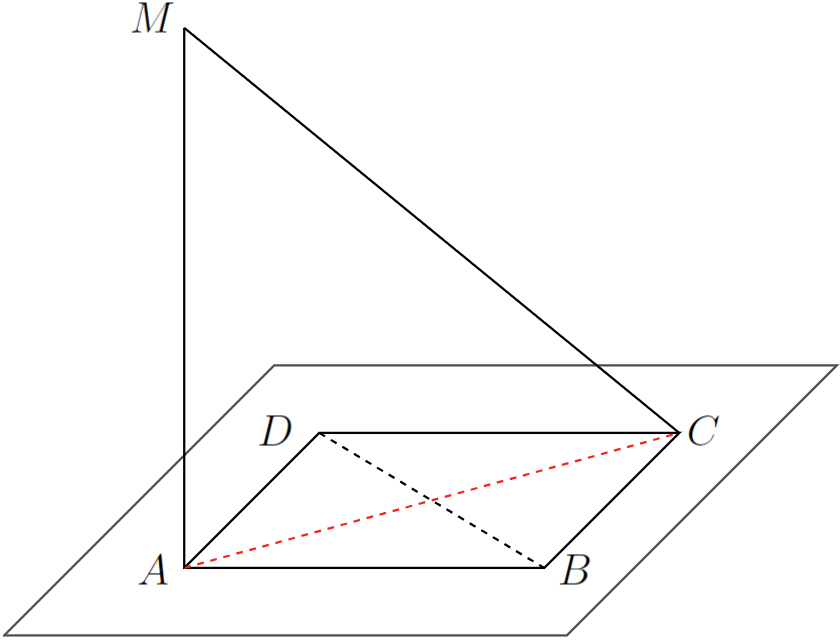
\includegraphics[width=0.4\textwidth]{垂线例10.png}
    \caption*{\texttt{例题}\ref{et:1-3-10}}
\end{wrapfigure}

给定平面,总有与它垂直的直线。反过来,给定一条直线,是否有与它垂直的平面呢?设直线的方向向量为$\mathbf{n}$,
我们来看与它垂直的向量有什么共同特征。
\begin{tm}\label{tm:1-3-60}
    所有与非零向量$\mathbf{n}$垂直的向量构成一个过原点的平面。    
\end{tm}
\begin{proof2}
设$\mathbf{n} = (n_x, n_y, n_z)$是非零向量,所以$n_x, n_y, n_z$不全为零。
设$n_x\neq 0$,则向量$P_1(-n_y, n_x, 0)$和$P_2(-n_z, 0, n_x)$都垂直于$\mathbf{n}$。
容易验证$P_1,P_2$线性无关,因此它们确定的平面$\gamma$垂直于$\mathbf{n}$。

另一方面,设$P$与非零向量$\mathbf{n}$垂直,下面证明$P$在平面$\gamma$中。

可以验证$P_1, P_2, \mathbf{n}$线性无关,因此是空间的一组基底。用消影法将它正交归一,
得到正交归一基$(Q_1, Q_2,\mathbf{m})$,其中$Q_1,Q_2$是$P_1, P_2$正交归一的结果,
是平面$\gamma$的正交归一基,$\mathbf{m}$是平面$\gamma$的法向量,因此$\mathbf{m}$、$\mathbf{n}$共线。
将$P$在$Q_1, Q_2,\mathbf{m}$上分解:
$$ P = p_1Q_1 + p_2Q_2 + p_m\mathbf{m}.$$
$P$垂直于$\mathbf{n}$,因此也垂直于$\mathbf{m}$。于是$\mathbf{m}\cdot P = 0$,
即$p_m = 0$。因此$P = p_1Q_1 + p_2Q_2$在平面$\gamma$中。
综上所述,所有与非零向量$\mathbf{n}$垂直的向量构成过原点的平面$\gamma$。

\end{proof2}

给定一条直线$l:\mathbb{R}\mathbf{a} + \mathbf{b}$及一点$P$,
与$\mathbf{a}$垂直的向量构成一个过原点的平面。
把该平面按$P$平移,就得到一个过$P$的平面。也就是说:
\begin{tm}\label{tm:1-3-70}
    过一点恰有一个平面与给定直线垂直。
\end{tm}

过空间的每一点,恰有一个平面与给定直线垂直。这些垂直于同一直线的平面,有什么特征呢?
\begin{tm}\label{tm:1-3-80}
    垂直于同一直线的平面,相互平行或重合。
\end{tm}
\begin{proof2}
    设平面$\gamma_1,\gamma_2$与直线$l$垂直,与$l$分别交于点$P_1,P_2$。过$P_1$在$\gamma_1$中作两条直线$m_1,m_2$,
    过$P_2$作$m_1$的平行线$n_1$,$n_1\perp l$,因此$n_1$在$\gamma_2$中。
    同理,过$P_2$作$m_2$的平行线$n_2$,$n_2$在$\gamma_2$中。
    因此根据定理\ref{tm:1-0-70},$\gamma_1$与$\gamma_2$平行或重合。
\end{proof2}

设非零向量$\mathbf{n} = (n_x, n_y, n_z)$,与它垂直的向量的集合,就是以下方程的解集。
$$ n_xx + n_yy + n_zz = 0. $$
任何过原点的平面,都有法向量,于是总可以写成三元一次方程的解集。
因此,过原点的平面,可以用一个三元一次方程定义。

不过原点的平面,可以看作过原点平面按同一向量平移得到。如果过原点平面上的点满足方程
$$ n_xx + n_yy + n_zz = 0, $$
那么按向量$B(x_b, y_b,z_b)$平移之后得到的点就满足方程:
$$ \mbox{}\qquad\qquad n_x(x - x_b) + n_y(y - y_b) + n_z(z - z_b) = 0. \quad\quad (*)$$
因此,任何平面总是某个三元一次方程的解集。反之,任何三元一次方程$ax+by+cz+d = 0$总能写成
$(*)$的形式,于是解集为某个平面。我们将$ax+by+cz+d = 0$称为平面的一般式,将$(*)$称为平面的点法式,
即经过$B(x_b, y_b,z_b)$且垂直于向量$\mathbf{n} = (n_x, n_y, n_z)$。

三元一次方程的解集是平面,因此,我们也用它来定义平面。
比如,$x$轴和$y$轴所在平面$Oxy$可以用方程$z = 0$定义,过点$(-2,10,3)$并与它平行的平面可以用$z = 3$定义。	

用方程来定义平面,可以得出更多结论。
比如,考虑到空间中两点$P_1(x_1, y_1, z_1)$和$P_2(x_2, y_2, z_2)$相等的点$P(x,y,z)$,这样的点满足方程:
$$ (x - x_1)^2 + (y - y_1)^2 + (z - z_1)^2 = (x - x_2)^2 + (y - y_2)^2 + (z - z_2)^2. $$
方程两边消去$x^2 + y^2 + z^2$,得到关于$x,y,z$的三元一次方程:
$$ 2(x_1-x_2)x + 2(y_1-y_2)y + 2(z_1-z_2)z = x_1^2+y_1^2+z_1^2 - x_2^2-y_2^2-z_2^2. $$
因此,到两点距离相等的点构成一个平面,称为这两点的\textbf{垂直平分面}。

再来看平面与平面的垂直关系。两个平面相互垂直,指它们的法向量相互垂直。
平行平面的法向量相同,所以如果平面与两平行平面中的一个垂直,那么与另一个也垂直。

显然,过平面中一点,有无数平面与它垂直。比如,过$x$轴和$y$轴所在平面$Oxy: z = 0$中的$(0,0,0)$点,
可以找到平面$x + y = 0$与它垂直。不仅如此,$x + 2y = 0$、$x + 3.3y = 0$、$2.6x - y = 0$等也都与它垂直。
但所有与它垂直的平面,都经过直线$\{(t,0,0) \, | \, t\in \mathbb{R}\} = \mathbb{R}\mathbf{e}_z$。

\begin{sk}
    \mbox{} \\
    \indent 1. 空间中,垂直于同一直线的平面平行或重合,垂直于同一平面的直线平行或重合。这性质和平面中直线的哪些性质相似?\\
    \indent 2. 空间中的直线能否表示为方程的解集?如果可以,是怎样的方程?
\end{sk}

\begin{xt}
    \mbox{} \\ 
    \indent 1. 设过点$P$的平面$\gamma = \{s\mathbf{u} + t\mathbf{v} + P \, | \, s,t\in\mathbb{R}\}$。\\
    \indent 1.1. 设$Q_1,Q_2$为平面$\gamma$中两点,用$\mathbf{u},\mathbf{v}$表示向量$\vv{Q_1Q_2}$。\\
    \indent 1.2. 证明:平面$\gamma$中任何直线的方向向量总是$\mathbf{u},\mathbf{v}$的线性组合。\\
    \indent 1.3. 证明:如果直线与平面中两条相交直线垂直,就垂直于这个平面。\\     
    \indent 2. 给定两个线性无关的向量$A,B$。\\
    \indent 2.1. 如果$A,B$是单位向量,证明$A+B \perp A-B$。\\
    \indent 2.2. 以第一问的结论为基础,给出另一种正交归一的方法。\\
    \indent 3. 求与$(2,-1,1)$、$(0,1,2)$垂直的单位向量。\\
    \indent 4. 求过$(1,0,0)$且垂直于$\mathbb{R}(0,1,0)+(1,-1,1)$的平面。\\
    \indent 4. 试将平面$\{s(1,-1,0) + t(-2,1,1) + (0,0,1) \, | \, s,t\in\mathbb{R}\}$表示为三元一次方程的解集。
\end{xt}


\section{垂线和距离}
了解了直线、平面之间的垂直关系,我们进一步来讨论点、直线、平面之间的距离。

平面中,求点到直线的距离,可以过点作直线的垂线,求点到垂足的距离。
给定点$A$和直线$l : \mathbb{R}\mathbf{v} + B$,过$A$作$l$的垂线,记垂足为$P = t\mathbf{v} + B$。
如果$\vv{AB}\perp\mathbf{v}$,那么$B=P$就是垂足,距离就是$|AB|$。
否则$P\neq B$,$\triangle ABP$是直角三角形,$\angle APB$是直角。向量$\vv{BP}$垂直于$\vv{AP}$,因此
$$ \vv{AP}\cdot \vv{BP} = 0.$$
即
$$ (t\mathbf{v} + B - A)\cdot t\mathbf{v} = 0.$$
解得$t = \frac{\mathbf{v}(A-B)}{\|\mathbf{v}\|^2}$。不妨设$\mathbf{v}$是单位向量,那么$t=\mathbf{v}\cdot(A-B)$。
于是$A$到$l$的距离为$|AP| = \| t\mathbf{v} + B - A\| = \| \vv{AB} - (\mathbf{v}\cdot \vv{AB})\mathbf{v}\|$。
直观来看,这表示$|AP| = |AB|\sin{\angle ABP}$。

求空间中一点到平面的距离,也和求点到直线距离类似,可以作点到平面的垂足,求点到垂足的距离。
具体来说,设平面$\gamma$经过点$B$,法向量为$\mathbf{n}$,点$A$到平面$\gamma$的垂线为:
$$ \mathbb{R}\mathbf{n} + A$$
设垂足为$P$,则$A$到平面$\gamma$的距离就是$|AP|$。

直线$AP$垂直于$\gamma$,因此也垂直于$\gamma$中的直线$BP$,于是$\triangle ABP$是直角三角形,
所以点$A$到平面的距离就是$|AP| = |AB|\cos{\angle ABP}$,也就是向量$\vv{AB}$和法向量$\mathbf{n}$的内积的绝对值,
或者说$|AB|$在法线$AP$上的投影的长度:
$$ |AP| = |\mathbf{n}\cdot \vv{AB}|. $$

接下来讨论直线与直线的距离。平面中,不相交的直线是平行直线。空间中,不相交直线的距离,包括平行和异面两种情况。平行直线的距离,计算方法和平面中类似。
下面讨论异面直线的距离。

考虑两条异面直线,它们的方向向量线性无关。因此,我们可以用定理\ref{tm:1-3-30}讨论与它们都垂直的直线。

设有异面直线$l_1:\mathbb{R}\mathbf{a}_1 + \mathbf{b}_1$、$l_2:\mathbb{R}\mathbf{a}_2 + \mathbf{b}_2$,
其中$\mathbf{a_1}, \mathbf{a}_2$是单位向量。
按照定义,$\mathbf{a}_1$和$\mathbf{a}_2$线性无关。根据定理\ref{tm:1-3-30},有单位向量$\mathbf{n}$与它们都垂直。
考虑以$\mathbf{n}$为方向的直线$m$,$m$与$l_1,l_2$都垂直。如果$m$与$l_1,l_2$都相交,就说$m$是$l_1,l_2$的\textbf{公垂线}。
下面我们来找出$l_1,l_2$的公垂线。

我们把$m$表示成$m: \mathbb{R}\mathbf{n} + r_1\mathbf{a}_1 + r_2\mathbf{a}_2$,设$m$与$l_1,l_2$的交点分别是:
\begin{align}
    P_1 = t_1\mathbf{a}_1 + \mathbf{b}_1 &= s_1\mathbf{n} + r_1\mathbf{a}_1 + r_2\mathbf{a}_2 \notag \\
    P_2 = t_2\mathbf{a}_2 + \mathbf{b}_2 &= s_2\mathbf{n} + r_1\mathbf{a}_1 + r_2\mathbf{a}_2  \notag
\end{align}
两点分别与$\mathbf{a_1}, \mathbf{a}_2,\mathbf{n}$求内积,得到:
$$
\left\{
\begin{array}[]{cl}
    t_1 + \mathbf{a}_1\cdot\mathbf{b}_1 &= r_1 + r_2\mathbf{a}_1\cdot\mathbf{a}_2 \\
    t_1\mathbf{a}_1\cdot\mathbf{a}_2 + \mathbf{a}_2\cdot\mathbf{b}_1 &= r_1\mathbf{a}_1\cdot\mathbf{a}_2 + r_2 \\
    t_2 + \mathbf{a}_2\cdot\mathbf{b}_2 &= r_1\mathbf{a}_1\cdot\mathbf{a}_2 + r_2 \\
    t_2\mathbf{a}_1\cdot\mathbf{a}_2 + \mathbf{a}_1\cdot\mathbf{b}_2 &= r_1 + r_2\mathbf{a}_1\cdot\mathbf{a}_2 \\
    \mathbf{n}\cdot\mathbf{b}_1 &= s_1 \\
    \mathbf{n}\cdot\mathbf{b}_2 &= s_2
\end{array}
\right.
$$
从前$4$个方程可以求出$t_1,t_2,r_1,r_2$唯一的一组解,于是可以得到直线$m$,
也就是说,异面直线$l_1,l_2$总有唯一的公垂线。我们称线段$P_1P_2$为$l_1,l_2$的\textbf{公垂线段}。

向量$\vv{P_1P_2}$与$\mathbf{n}$共线。从后两个方程可以解出$s_1,s_2$,因此线段$P_1P_2$的长度是:
\begin{align}
    |P_1P_2| = \|P_2 - P_1\| &= \|s_1\mathbf{n} + r_1\mathbf{a}_1 + r_2\mathbf{a}_2 - (s_2\mathbf{n} + r_1\mathbf{a}_1 + r_2\mathbf{a}_2)\| \notag \\
    &= \| (s_1 - s_2)\mathbf{n} \| \notag \\
    &= |\mathbf{n}\cdot(\mathbf{b}_1 - \mathbf{b}_2)|. \notag
\end{align}
在$l_1,l_2$上各取一点:$Q_1 = P_1 + q_1\mathbf{a_1}$、$Q_2 = P_2 + q_2\mathbf{a}_2$,则:
\begin{align}
    \vv{Q_1Q_2} = P_2 + q_2\mathbf{a}_2 - (P_1 + q_1\mathbf{a_1}) = \vv{P_1P_2}  + (q_2\mathbf{a}_2 - q_1\mathbf{a_1}). \notag 
\end{align}
而$\vv{P_1P_2} = (s_1 - s_2)\mathbf{n} \perp q_2\mathbf{a}_2 - q_1\mathbf{a_1}$,所以,根据勾股定理,
\begin{align}
    |Q_1Q_2|^2 = |P_1P_2|^2 + \|q_2\mathbf{a}_2 - q_1\mathbf{a_1}\|^2 \geqslant |P_1P_2|^2. \notag 
\end{align}
这说明$l_1$上的点到$l_2$上的点的距离总大于等于$|P_1P_2|$。
我们把$|P_1P_2|$称为\textbf{异面直线的距离}。

直线和平面的距离,也可以用公垂线定义。设直线$l:\mathbb{R}\mathbf{v} + A$平行于平面$\gamma$,
我们可以找出与$l$和$\gamma$都垂直的直线,称为它们的公垂线。具体来说,过$A$点有唯一一条与$\gamma$垂直的直线:
$$ m:\mathbb{R}\mathbf{n} + A $$
其中$\mathbf{n}$是$\gamma$的法向量。设$m$与$\gamma$交于点$P$,过$P$作$l$的平行线$n:\mathbb{R}\mathbf{v} + P$。
由于$l\parallel\gamma$,所以$n$在$\gamma$中。于是$m\perp n$,即$m\perp l$。
我们说$m$是直线$l$和平面$\gamma$的\textbf{公垂线}。

显然,直线和平面的公垂线不是唯一的。过直线上任一点,都恰有一条公垂线。定义直线和平面的距离为公垂线段$AP$的长度$|AP|$。
我们可以用求点到直线距离的方式,求出$|AP|$。比如,设平面经过点$B$,则$|AP| = |\mathbf{n}\cdot \vv{AB}|.$

最后讨论平行平面之间的距离。垂直于同一直线的平面相互平行或重合,因此,相互平行的平面,法向量应该相同。
这一点并不难证明。设平面$\gamma_1,\gamma_2$相互平行。在$\gamma_1$中取相交直线
$\mathbb{R}\mathbf{a}_1 + \mathbf{b}_1$、$\mathbb{R}\mathbf{a}_2 + \mathbf{b}_1$,
过$\gamma_2$中一点$\mathbf{b}_2$作它们的平行线,则两条平行线都在$\gamma_2$中,
且方向向量分别为$\mathbf{a}_1,\mathbf{a}_2$。
因此,$\gamma_1,\gamma_2$可以写成:
\begin{align}
    \gamma_1 = \mathbb{R}\mathbf{a}_1 + \mathbb{R}\mathbf{a}_2 + \mathbf{b}_1 \notag \\
    \gamma_2 = \mathbb{R}\mathbf{a}_1 + \mathbb{R}\mathbf{a}_2 + \mathbf{b}_2 \notag
\end{align}
它们的法向量都可从$\mathbf{a}_1,\mathbf{a}_2$通过消影法得到,因此是同一个单位向量$\mathbf{n}$。

考虑直线$\mathbb{R}\mathbf{n}$与$\gamma_1,\gamma_2$的交点$P_1,P_2$,可以得到:
$$
\begin{array}[]{c}
    P_1 = r_1\mathbf{n} = s_1\mathbf{a}_1 + t_1\mathbf{a}_2 + \mathbf{b}_1 \\
    P_2 = r_2\mathbf{n} = s_2\mathbf{a}_1 + t_2\mathbf{a}_2 + \mathbf{b}_2 
\end{array} 
$$
类似异面直线的情况,通过对$\mathbf{n}$求内积,我们得到
$$
\begin{array}[]{c}
    r_1 = \mathbf{n}\cdot\mathbf{b}_1 \\
    r_2 = \mathbf{n}\cdot\mathbf{b}_2 
\end{array}
$$
因此,两交点的距离为:
$$ |P_1P_2| = \| r_2\mathbf{n} - r_1\mathbf{n}\| = |\mathbf{n}\cdot(\mathbf{b}_1 - \mathbf{b}_2)|. $$
在$\gamma_1,\gamma_2$上各取一点:$Q_1 = P_1 + q_{1,1}\mathbf{a_1} + q_{1,2}\mathbf{a}_2$、
$Q_2 = P_2 + q_{2,1}\mathbf{a_1} + q_{2,2}\mathbf{a}_2$,则:
\begin{align}
    \vv{Q_1Q_2} = \vv{P_1P_2}  + (q_{2,1}\mathbf{a_1} + q_{2,2}\mathbf{a}_2 - q_{1,1}\mathbf{a_1} - q_{1,2}\mathbf{a}_2). \notag 
\end{align}
而$\vv{P_1P_2} = (r_2 - r_1)\mathbf{n} \perp q_{2,1}\mathbf{a_1} + q_{2,2}\mathbf{a}_2 - q_{1,1}\mathbf{a_1} - q_{1,2}\mathbf{a}_2$,所以,根据勾股定理,
\begin{align}
    |Q_1Q_2|^2 = |P_1P_2|^2 + \|q_{2,1}\mathbf{a_1} + q_{2,2}\mathbf{a}_2 - q_{1,1}\mathbf{a_1} - q_{1,2}\mathbf{a}_2\|^2 \geqslant |P_1P_2|^2. \notag 
\end{align}
这说明$\gamma_1$上的点到$\gamma_2$上的点的距离总大于等于$|P_1P_2|$。
我们把$|P_1P_2|$称为\textbf{平行平面的距离}。

\begin{xt}
    \mbox{} \\
    \indent 1. 求点$(2,0,1)$到平面$x +2y - 5z + 1 = 0$的距离。\\
    \indent 2. 求点$(1,1,-1)$到直线$\mathbb{R}(0,3,-1) + (1,-2,1)$的距离。\\
    \indent 3. 求异面直线$\mathbb{R}(0,1,1)+(1,-1,0)$、$\mathbb{R}(1,0,-1)+(0,1,-1)$的公垂线及距离。\\
    \indent 4. 求直线$\mathbb{R}(1,2,-1) + (0,1,1)$到平面$x + y + 3z - 1 = 0$的距离。\\
    \indent 5. 求平行平面$x-y+z=1$和$x-y+z=-1$的距离。\\
    \indent 6. 点$(1,a,a+2)$到平面$2x - y - z + 2 = 0$和$x + 3y - 4z = 0$的距离相等,求$a$的值。
\end{xt}

\begin{appendix}

\chapter{空间形的表示法}

为了方便讨论空间形,我们希望在纸面上快速便捷地表示空间中的点、直线、平面等基本形状。
讨论平面形状时,我们自然地将纸面作为形状所在的平面。讨论空间中的形状时,
我们没法在纸面上完整表示立体图形,所以需要一套统一约定的折衷方法,方便交流。
我们把这样的方法称为\textbf{作图法}或\textbf{画法}。

人类自古以来就在探索作图法。距今两万年的壁画上,就有用线条表示动物和地形的创作。
人类对作图法的探索有两个方向,一个致力于在平面上真实地还原人眼看到的景物,
另一个致力于用简练记号表述空间中的对象。前者发展出以透视法为基础的艺术绘画技法,
后者发展出以地图、工程图等为代表的实用绘图技法。
下面介绍的属于后者,是数学中一种常用的简便作图法。

\section{在空间中画平面}

空间中的平面是没有边界的。为了在有限的纸面上表示平面,我们选用一定的形状框定边界,表示一个平面,
称为平面的\textbf{示形}。要注意的是,这样表示的平面其实是平面的一部分,但不妨碍我们想象它是无边际延伸开来的。

我们约定用常见的平行四边形表示平面。平行四边形的长边长度一般介于短边长度的$1.5$至$3$倍之间,
长短边的锐角夹角一般是$45$度角。

一般来说,水平位置的平面(称为\textbf{水平面}),用上下对边水平的平行四边形表示,竖直位置的平面(称为竖立面),
用左右对边竖直的平行四边形表示。矩形一般表示正对视线的竖直平面。完全侧对视线的竖直平面,用$45$度角的上下对边表示。

平面的名字一般标记在示形内部,靠近其某个顶点。

当一个平面示形的一部分被其它平面遮住时,我们用虚线表示被遮住部分的边界。如果虚线使得画面过于繁杂难辨,
可以连虚线也不画。

用平行四边形表示平面,意味着我们降低了对真实性的要求,比如舍弃了近大远小的性质。
因此作出的图形往往“不真实”。例如,一个水平面,我们看不出它到底位于我们上方还是下方。
为此我们约定,\textbf{所有水平面均处于视线下方},即我们总在俯视这些平面。
这样,水平面靠下的点离我们较近,靠上的点离我们较远。

\section{在水平面中画平面图形}

已知一个平面形的样子,如何把它画在空间中某个水平面里?

我们把平面形所在的图称为平面图,把要画的图称为立体图。首先在立体图中画出水平面。
为了方便,设示形的水平边长度为非水平边的$2$倍,夹角为$45$度。这个比例系数和夹角在下面画平面图形时将一直使用。

选择平面图中一条线段、射线或直线作为\textbf{水平线}。把它画进立体图时,画成水平方向,
长度不变。与它平行的线段、射线、直线,也画成水平方向,线段长度不变。

平面图中垂直于水平线的线段、射线或直线(称为\textbf{纵直线}),把它画进立体图时,
画成与平面非水平对边平行的方向($45$度角),线段的长度要除以$2$。

要将平面图中一点画进立体图中,可以先在平面图中作它到水平线和纵直线的垂线。
这样,该点就成了水平线和纵直线的交点,于是可以在立体图中作出对应的点。

平面图中其它位置的线段、射线或直线,在其中取两点(线段一般取端点,射线取端点和较远一点,
直线取较远两点)。将两点按上述方法画进立体图中,再连出对应的线段、射线或直线。

约定平面图中的上下左右关系在立体图中不变。但立体图中的上下关系应理解为前后关系,
即靠上的在后(较远),靠下的在前(较近)。

\section{在一般平面中画平面图形}

在一般平面中画平面图形是复杂的操作。从原则上来说,违背了简便作图法的精神,
容易产生既不简便、真实性也低的困境。因此,如果可以选择在水平面中画平面图形,最好不要在非水平面中画。

和在水平位置的平面中画平面图形的方法类似,我们需要在立体图中示形的对边中选择一个\textbf{主边}和一个\textbf{副边}。
水平面中,我们选择水平方向的对边为主边,非水平方向的对边为副边。一般平面中,需要自行选择边和副边。
主边长度和副边长度之比称为\textbf{斜变系数},比如水平位置平面的斜变系数为$2$。

选定之后,主方向将对应平面图中的水平线,副方向将对应平面图中的纵直线。
平面图中平行于水平线的线段、射线、直线,按主边方向画出,线段长度不变。
平面图中垂直于水平线的线段、射线、直线,按副边方向画出,线段长度要除以斜变系数。

要将平面图中一点画进立体图中,可以先在平面图中作它到水平线和纵直线的垂线。
这样,该点就成了水平线和纵直线的交点,于是可以在立体图中作出对应的点。

平面图中其它位置的线段、射线或直线,在其中取两点(线段一般取端点,射线取端点和较远一点,
直线取较远两点)。将两点按上述方法画进立体图中,再连出对应的线段、射线或直线。

把平面图形画到非水平面中的时候,平面图中的上下左右关系在立体图中可能改变。
为此,作图时需要注意保持一致性,否则将产生错误的结果。

\section{画空间直角坐标系}

以上作图法中,其实已经用到了坐标系的想法。比如,平面图中的水平线可以看作坐标轴横轴,
纵直线可以看作坐标轴纵轴。我们把平面图中一点画到立体图中时,过它作到水平线和纵直线的垂线,实际上就在确定它的坐标。

我们可以直接在立体图中画出直角坐标系。一般来说,选定的基底$\mathbf{e}_x,\mathbf{e}_y,\mathbf{e}_z$,
表示三个两两垂直的单位向量,对应三条射线。在立体图中,直角坐标系有多种画法。

选定一点为原点,过原点往右作水平射线,这条射线可以是$x$轴或$y$轴正半部分。如果设它为$x$轴正半,
那么过原点往右上$45$度角作射线,是为$y$轴正半;如果设它为$y$轴正半,那么过原点往左下$45$度角作射线,
是为$x$轴正半。最后过原点往上作竖直射线,是为$z$轴正半。这种画法称为\textbf{右手正斜式}。
将$x$轴和$y$轴互换,则称为\textbf{左手正斜式}。

另一种画法从$z$轴开始。过原点往上作竖直射线,是为$z$轴正半。将其顺时针旋转$120$度,得到$x$轴正半;
顺时针再旋转$120$度,得到$y$轴正半。这种画法称为\textbf{右手对称式}。将$x$轴和$y$轴互换,则称为\textbf{左手对称式}。

更一般的画法则继续向透视法靠拢。比如参考两点透视画出水平位置的矩形,以此确定$x$轴和$y$轴。
我们不在此展开,只介绍正斜式画法。

正斜式画法与前面的平行四边形表示法兼容。从左下为$x$轴的右手对称式出发,容易看出,
$Oxy$就是水平面。为了方便,我们在它的示形基础上画坐标系。选好长短边长度后,水平上边就是$y$轴,
非水平的左边就是$x$轴。将代表射线的箭头画在平行四边形对应的顶点,然后将这两边等分,标上坐标刻度。
$z$轴(竖轴)按$y$轴长度标上刻度。朝反方向延伸可以画出各坐标轴的负半部分,并标上刻度。

按照坐标轴刻度,可以找出$Oxy$中点的位置。比如,要画出坐标为$(1,2,0)$的点,可以在$x$轴找到刻度为$1$的点,
过它作平行于$y$轴的直线(水平线);在$y$轴找到刻度为$2$的点,过它作平行于$x$轴的直线;
两线交点就是坐标为$(1,2,0)$的点。

对于不在$Oxy$中的点,可以先画出它在$Oxy$上的投影点。比如,要画出坐标为$(1,2,3)$的点,
可以先画出$(1,2,0)$,然后过它作平行于$z$轴的直线。由于往上为$z$轴正向,所以对于正数$3$,
往上数三个单位长度,即为$(1,2,3)$。如果要画坐标为$(1,2,-3)$的点,则向下数三个单位长度。
为了清楚表明点在空间中的位置,可以保留投影点,并将投影点与$x$轴、$y$轴用虚线连线,将目标点和投影点用虚线连线。

\chapter{空间向量与公理}

下面验证:根据向量定义的点、直线、平面符合平面公理、平直公理、交面公理和补充的平行公理。

\section{平面公理}
首先来看平面公理。任取不共线三点$A,B,C$,则$A-C,B-C$线性无关,
因此$ \{sA+tB+(1 - s - t)C \, | \,s, t\in\mathbb{R}\}$是$A,B,C$确定的平面。

\section{平直公理}
再来看平直公理。
如果点$P,Q$在平面$ \{sA+tB+(1 - s - t)C \, | \, s,t\in\mathbb{R}\}$中,那么存在$s_1, t_1, s_2, t_2$使得
\begin{align}
P &= s_1A + t_1B + (1 - s_1 - t_1)C \notag \\
Q &= s_2A + t_2B + (1 - s_2 - t_2)C \notag 
\end{align}
直线$PQ$是集合$\{uP+(1-u)Q \, | \, u\in \mathbb{R}\}$,其中任一点$U = uP+(1-u)Q$可以用$A,B,C$表示为
\begin{align}
U &= uP+(1-u)Q \notag \\
&= (us_1 + (1-u)s_2)A + (ut_1 + (1-u)t_2)B + (u(1 - s_1 - t_1) + (1-u)(1 - s_2 - t_2))C  \notag \\
&= (us_1 + (1-u)s_2)A + (ut_1 + (1-u)t_2)B + (1 - (us_1 + (1-u)s_2) - (ut_1 + (1-u)t_2))C \notag
\end{align}
因此$U$在平面$ABC$中。这说明向量表示的空间符合平直公理。

\section{交面公理}
接下来验证交面公理。
如果两平面$\gamma_1, \gamma_2$交于点$C$,记$\gamma_1 = \mathbb{R}A_1+\mathbb{R}B_1+C$,$\gamma_2 = \mathbb{R}A_2+\mathbb{R}B_2+C$。
其中$(A_1,B_1)$线性无关,$(A_2,B_2)$线性无关。两平面公共点可以表示为让以下等式成立的$s_1,t_1,s_2,t_2$:
$$ s_1A_1+t_1B_1+C = s_2A_2+t_2B_2+C. $$
以上等式可以转为:
$$ s_1A_1+t_1B_1 - s_2A_2 - t_2B_2 = \mathbf{0}. $$
根据空间的根本性质,四个向量总是线性相关。所以存在不全为零的四个实数$s_1,t_1,s_2,t_2$使上式成立。
由于$(A_1,B_1)$线性无关,$(A_2,B_2)$线性无关,所以$s_1A_1+t_1B_1$和$s_2A_2 + t_2B_2$为零向量时,
$s_1,t_1,s_2,t_2$必然全为零。然而$s_1,t_1,s_2,t_2$不全为零,所以$s_1A_1+t_1B_1$和$s_2A_2 + t_2B_2$不为零向量。
于是这时$s_1A_1+t_1B_1+C = s_2A_2+t_2B_2+C\neq C$是两平面另一个公共点。这说明向量表示的空间符合交面公理。

\section{平行公理}
我们主要验证平行线共面的性质。
平面中,两条直线平行,当且仅当它们的线性部分是同一条过原点的直线。我们用这个方法来判定空间中直线的平行关系。设有两直线$l_1\parallel l_2$,那么它们是同一条过原点的直线平移而成:
\begin{align}
l_1: & \,\,\, \mathbb{R}\mathbf{a} + \mathbf{b}_1 \notag \\
l_2: & \,\,\, \mathbb{R}\mathbf{a} + \mathbf{b}_2\notag
\end{align}
所以$l_1,l_2$都在平面:$\gamma = \mathbb{R}\mathbf{a} + \mathbb{R}(\mathbf{b}_1 - \mathbf{b}_2) + \mathbf{b}_2$中。
对任意$t\in\mathbb{R}$,$l_1$中的点$t\mathbf{a} + \mathbf{b}_1 = t\mathbf{a} + 1\cdot(\mathbf{b}_1 - \mathbf{b}_2) + \mathbf{b}_2 \in \gamma$;
$l_2$中的点$t\mathbf{a} + \mathbf{b}_2 = t\mathbf{a} + 0\cdot(\mathbf{b}_1 - \mathbf{b}_2) + \mathbf{b}_2 \in \gamma$。
这说明,两条平行直线总在同一平面内,即向量表示的空间符合补充后的平行公理。

\end{appendix}





\end{document}